\chapter*{Programme officiel}

\section*{Programme officiel}

Exprimer un algorithme dans un langage de programmation a pour but de le rendre exécutable par une machine dans un contexte donné. La découverte de l'architecture des machines et de leur système d'exploitation constitue une étape importante.

Les circuits électroniques sont au cœur de toutes les machines informatiques. Les réseaux permettent de transmettre l'information entre machines. Les systèmes d'exploitation gèrent et optimisent l'ensemble des fonctions de la machine, de l'exécution des programmes aux entrées-sorties et à la gestion d'énergie.

On étudie aussi le rôle des capteurs et actionneurs dans les entrées-sorties clavier, interfaces graphiques et tactiles, dispositifs de mesure physique, commandes de machines, etc.

{\centering\begin{tabular}{|L{3cm}|L{5.5cm}|L{6cm}|}\hline
\cellcolor{bo}\bfseries\textcolor{white}{Contenus}&
\cellcolor{bo}\bfseries\textcolor{white}{Capacités attendues}&
\cellcolor{bo}\bfseries\textcolor{white}{Commentaires}\\ \hline
Modèle d'architecture séquentielle (von Neumann)
&
Distinguer les rôles et les caractéristiques des différents constituants d'une machine.

Dérouler l'exécution d'une séquence d'instructions simples du type langage machine.
&
La présentation se limite aux concepts généraux.

On distingue les architectures monoprocesseur et les architectures multiprocesseur.

Des activités débranchées sont proposées.

Les circuits combinatoires réalisent des fonctions booléennes.\\ \hline
Transmission de données dans un réseau

Protocoles de communication

Architecture d'un réseau

&
Mettre en évidence l'intérêt du découpage des données en paquets et de leur encapsulation.

Dérouler le fonctionnement d'un protocole simple de récupération de perte de paquets (bit alterné).

Simuler ou mettre en œuvre un réseau.
&
Le protocole peut être expliqué et simulé en mode débranché.

Le lien est fait avec ce qui a été vu en classe de seconde sur le protocole TCP/IP.

Le rôle des différents constituants du réseau local de l'établissement est présenté.\\ \hline
Systèmes d'exploitation
&
Identifier les fonctions d'un système d'exploitation.

Utiliser les commandes de base en ligne de commande.

Gérer les droits et permissions d'accès aux fichiers.
&
Les différences entre systèmes d'exploitation libres et propriétaires sont évoquées.

Les élèves utilisent un système d'exploitation libre.

Il ne s'agit pas d'une étude théorique des systèmes d'exploitation.\\ \hline
Périphériques d'entrée et de sortie

Interface Homme-Machine (IHM)
&
Identifier le rôle des capteurs et actionneurs.

Réaliser par programmation une IHM répondant à un cahier des charges donné.
&
Les activités peuvent être développées sur des objets connectés, des systèmes embarqués ou robots.\\ \hline
\end{tabular}\par}


\chapter{Modèle d'architecture}

\section{Qu'est-ce qu'un ordinateur ?}


\noindent\date{1945} Le mathématicien John von Neumann élabore la première description d'un ordinateur. On peut la simplifier ainsi :

\begin{center}\begin{tikzpicture}
\node[text width = 3cm, draw, align=center](A){\raisebox{-1ex}{\rule{0pt}{4ex}}Processeur};
\node[text width = 3cm, draw, align=center, xshift=2.5cm](B)at(A.east){\raisebox{-1ex}{\rule{0pt}{4ex}}Mémoire};
\node[text width = 3cm, draw, align=center, xshift=2.5cm](C)at(B.east){\raisebox{-1ex}{\rule{0pt}{4ex}}Entrées/Sorties};
\node[text width = 12cm, draw, align=center, yshift=-1cm, double arrow](D)at(B.south){Bus de communication};
\draw(A.south)--++($(D.north)-(B.south)$);
\draw(B.south)--++($(D.north)-(B.south)$);
\draw(C.south)--++($(D.north)-(B.south)$);
\end{tikzpicture}\end{center}

\Cours{{\bfseries Ordinateur}

Un ordinateur est une machine \emph{électronique} capable d'exécuter des \emph{instructions} effectuant des \emph{opérations} sur des \emph{nombres}.}

\subsection{Entrées/sorties}

\Cours{{\bfseries Entrées/sorties}

\begin{itemize}
    \item Un périphérique d'entrée permet de fournir des informations au système. 
    
    Exemples : Clavier, souris, scanner, micro, etc.
    \item Un périphérique de sortie permet de faire sortir des informations du système.
    
    Exemples : Écran, imprimante, haut-parleurs, etc.
    \item Un périphérique d'entrée/sortie permet l'échange d'informations dans les deux sens.
    
    Exemples : Clé USB, Carte son, carte réseau, etc.
\end{itemize}}

\subsection{Mémoires}

\Cours{{\bfseries Mémoire vie / Mémoire morte}

\begin{itemize}
    \item La mémoire vive ou temporaire est celle des barrettes de RAM (Random Access Memory), qui ne persiste pas hors tension.
    \item La mémoire morte ou persistante est celle du disque dur (Hard Drive), qui permet une mémorisation permanente.
\end{itemize}}

La mémoire vive est indispensable pour sa vitesse d'accès ($\approx 10$ns contre $\approx 5$ms pour la mémoire morte) et la mémoire morte est indispensable pour sa persistance.

De nos jours, les processeurs eux-mêmes sont dotés de leur propre petite mémoire vive, dite mémoire cache, pour augmenter les vitesses d'accès ($\approx 5$ns). Ils fonctionnent par ailleurs en manipulant de touts petits espaces mémoires appelés registres, encore plus rapides ($\approx 1$ns).



\subsection{Processeur}

\Cours{{\bfseries Processeur}

Le processeur est le composant électronique qui permet d'effectuer les calculs.
}

L'élément constitutif de base est le \emph{transistor}, sorte d'interrupteur, contrôlé, qui permet, ou non, de laisser passer le courant, donc aboutissant à deux états possibles : 0 ou 1. Le processeur ne travaille fondamentalement qu'avec \emph{deux chiffres}, donc avec des \emph{nombres binaires}.

\begin{center}\begin{tikzpicture}
\node(A){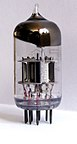
\includegraphics[scale=0.5]{images/tube.jpg}};
\node[yshift=-1.5cm]at(A){tube};
\node[xshift=3cm](B)at(A){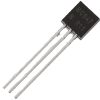
\includegraphics[scale=0.5]{images/transistor.png}};
\node[yshift=-1.5cm]at(B){transistor};
\node[xshift=3cm](C)at(B){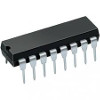
\includegraphics[scale=0.5]{images/ci.jpg}};
\node[yshift=-1.5cm]at(C){circuit itégré};
\end{tikzpicture}\end{center}

\noindent\date{1943} Le premier ordinateur, le Colossus était conçu à partir de tubes électroniques.

De nos jours, les transistors des processeurs ne font que quelques nanomètres et se comptent en milliards.
Combiner plusieurs transistors permet la création de \emph{circuits logiques}. Il en existe de deux types :

\begin{itemize}
	\item les circuits combinatoires, si les sorties ne sont fonction que des entrées.
	\item les circuits séquentiels, si les sorties dépendent également du temps et des états antérieurs.
\end{itemize}
\section{Circuits combinatoires}

\subsection{Porte non}
Le circuit combinatoire le plus simple celui qui permet de changer d'état :

\begin{itemize}
	\item Si l'entrée est $E=1$ alors la sortie est $S = 0$
	\item Si l'entrée est $E=0$ alors la sortie est $S = 1$
\end{itemize}

On identifie 0 à << faux >> et 1 à << vrai >> et ce circuit correspond alors à une négation : ce qui était vrai devient faux et ce qui était faux devient vrai. On appelle ce circuit une << porte non >> :


\begin{center}
\begin{multicols}{2}
Porte non

\begin{tikzpicture}
    \draw node[not port](not) {}; 
    \draw (not.out)--++(0.25,0)node[right]{$S$}; 
    \draw (not.in)--++(-0.25,0)node[left]{$E$};
\end{tikzpicture}

Table de vérité :

\begin{tabular}{c|c}
$E$ & $S$ \\
\hline
$0$ & $1$ \\
$1$ & $0$ \\
\end{tabular}
\end{multicols}
\end{center}

{\bfseries Pour aller plus loin : } ce circuit n'est composé que de deux transistors :

\ctikzset{tripoles/mos style/arrows}

nMOS \quad \begin{tikzpicture}[baseline=(G.base)]
\node[nmos](nmos){};
\node[left](G)at(nmos.G){$G$};
\node[above]at(nmos.D){$D$};
\node[below]at(nmos.S){$S$};
\end{tikzpicture}
\qquad équivalent à : \quad
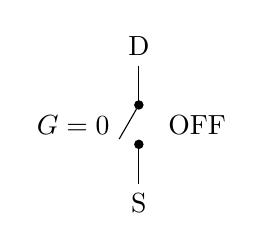
\begin{tikzpicture}[baseline=(G.base)]
\draw[](0,0)node[above]{D}--++(0,-0.5cm)node[inner sep = 0,circle,draw,fill=black](I){\rule{3pt}{0pt}};
\draw(I)--++(-120:0.5cm);
\draw[](0,-1.5cm)node[below]{S}--++(0,0.5cm)node[inner sep = 0,circle,draw,fill=black]{\rule{3pt}{0pt}};
\node[left](G)at(-0.25cm,-0.75cm){$G=0$};
\node[right](G)at(0.25cm,-0.75cm){OFF};
\end{tikzpicture}
\qquad
\begin{tikzpicture}[baseline=(G.base)]
\draw[](0,0)node[above]{D}--++(0,-0.5cm)node[inner sep = 0,circle,draw,fill=black](I){\rule{3pt}{0pt}};
\draw(I)--++(-90:0.5cm);
\draw[](0,-1.5cm)node[below]{S}--++(0,0.5cm)node[inner sep = 0,circle,draw,fill=black]{\rule{3pt}{0pt}};
\node[left](G)at(-0.25cm,-0.75cm){$G=1$};
\node[right](G)at(0.25cm,-0.75cm){ON};
\end{tikzpicture}


pMOS \quad \begin{tikzpicture}[baseline=(G.base)]
\node[pmos,emptycircle](pmos){};
\node[left](G)at(pmos.G){$G$};
\node[below]at(pmos.D){$D$};
\node[above]at(pmos.S){$S$};
\end{tikzpicture}
\qquad équivalent à : \quad
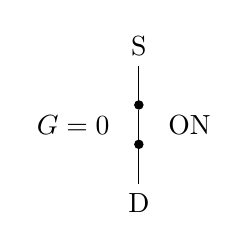
\begin{tikzpicture}[baseline=(G.base)]
\draw[](0,0)node[above]{S}--++(0,-0.5cm)node[inner sep = 0,circle,draw,fill=black](I){\rule{3pt}{0pt}};
\draw(I)--++(-90:0.5cm);
\draw[](0,-1.5cm)node[below]{D}--++(0,0.5cm)node[inner sep = 0,circle,draw,fill=black]{\rule{3pt}{0pt}};
\node[left](G)at(-0.25cm,-0.75cm){$G=0$};
\node[right](G)at(0.25cm,-0.75cm){ON};
\end{tikzpicture}
\qquad
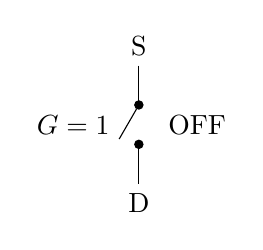
\begin{tikzpicture}[baseline=(G.base)]
\draw[](0,0)node[above]{S}--++(0,-0.5cm)node[inner sep = 0,circle,draw,fill=black](I){\rule{3pt}{0pt}};
\draw(I)--++(-120:0.5cm);
\draw[](0,-1.5cm)node[below]{D}--++(0,0.5cm)node[inner sep = 0,circle,draw,fill=black]{\rule{3pt}{0pt}};
\node[left](G)at(-0.25cm,-0.75cm){$G=1$};
\node[right](G)at(0.25cm,-0.75cm){OFF};
\end{tikzpicture}

\begin{tikzpicture}[baseline=(E.base)]
\node[pmos,emptycircle](pmos){};
\node[nmos, yshift=-1.5cm](nmos)at(pmos){};
\node[above]at(pmos.S){1 (alim)};
\node[below]at(nmos.S){0 (mass)};
\draw(pmos.G)--(nmos.G);
\draw($0.5*(pmos.G)+0.5*(nmos.G)$)--++(-0.25cm,0)node(E)[left]{$E$};
\draw($0.5*(pmos.D)+0.5*(nmos.D)$)--++(0.25cm,0)node[right]{$S$};
\end{tikzpicture}\qquad donne : \quad
\begin{tikzpicture}[baseline=(E.base)]
\draw[](0,0)node[above]{1}--++(0,-0.5cm)node[inner sep = 0,circle,draw,fill=black](I){\rule{3pt}{0pt}};
\draw(I)--++(-90:0.5cm)node[inner sep = 0,circle,draw,fill=black]{\rule{3pt}{0pt}}
     --++(0cm,-0.5cm)node[left=1cm](E){$E=0$}
     --++(0cm,-0.5cm)node[inner sep = 0,circle,draw,fill=black]{\rule{3pt}{0pt}}
     --++(-120:0.5cm);
\draw(0cm,-2.5cm)node[inner sep = 0,circle,draw,fill=black]{\rule{3pt}{0pt}}--++(0,-0.5cm)node[below]{0};
\draw(E.east)--++(0.25cm,0)|-++(0.25,0.75)node[inner sep = 0,circle,draw,fill=white](I){\rule{3pt}{0pt}};
\draw(E.east)++(0.25cm,0)|-++(0.25,-0.75);
\draw(E.east)++(1cm,0)--++(0.5cm,0)node[right]{$S=1$};
\end{tikzpicture}
\qquad
\begin{tikzpicture}[baseline=(E.base)]
\draw[](0,0)node[above]{1}--++(0,-0.5cm)node[inner sep = 0,circle,draw,fill=black](I){\rule{3pt}{0pt}};
\draw(I)--++(-120:0.5cm);
\draw(I)++(0,-0.5cm)node[inner sep = 0,circle,draw,fill=black]{\rule{3pt}{0pt}}
     --++(0cm,-0.5cm)node[left=1cm](E){$E=1$}
     --++(0cm,-0.5cm)node[inner sep = 0,circle,draw,fill=black]{\rule{3pt}{0pt}}
     --++(-90:0.5cm);
\draw(0cm,-2.5cm)node[inner sep = 0,circle,draw,fill=black]{\rule{3pt}{0pt}}--++(0,-0.5cm)node[below]{0};
\draw(E.east)--++(0.25cm,0)|-++(0.25,0.75)node[inner sep = 0,circle,draw,fill=white](I){\rule{3pt}{0pt}};
\draw(E.east)++(0.25cm,0)|-++(0.25,-0.75);
\draw(E.east)++(1cm,0)--++(0.5cm,0)node[right]{$S=0$};
\end{tikzpicture}


\subsection{Portes et / ou / ou exclusif}

Les portes logiques suivantes admettent deux entrées et une sortie.

\begin{center}
\begin{multicols}{3}
Porte et

\medskip

\begin{tikzpicture}
    \draw node[and port](and) {}; 
    \draw (and.out)--++(0.25,0)node[right]{$S$}; 
    \draw (and.in 1)--++(-0.25,0)node[left]{$E_1$};
    \draw (and.in 2)--++(-0.25,0)node[left]{$E_2$};
\end{tikzpicture}

\pythoninline{S = E1 & E2}

\medskip

\begin{tabular}{cc|c}
$E_1$ & $E_2$ & $S$ \\
\hline
$0$ & $0$ & $0$ \\
$0$ & $1$ & $0$\\
$1$ & $0$ & $0$ \\
$1$ & $1$ & $1$\\
\end{tabular}

\columnbreak
Porte ou

\medskip

\begin{tikzpicture}
    \draw node[or port](or) {}; 
    \draw (or.out)--++(0.25,0)node[right]{$S$}; 
    \draw (or.in 1)--++(-0.25,0)node[left]{$E_1$};
    \draw (or.in 2)--++(-0.25,0)node[left]{$E_2$};
\end{tikzpicture}

\pythoninline{S = E1 | E2}

\medskip

\begin{tabular}{cc|c}
$E_1$ & $E_2$ & $S$ \\
\hline
$0$ & $0$ & $0$ \\
$0$ & $1$ & $1$\\
$1$ & $0$ & $1$ \\
$1$ & $1$ & $1$\\
\end{tabular}

\columnbreak

Porte ou  exclusif

\medskip

\begin{tikzpicture}
    \draw node[xor port](xor) {}; 
    \draw (xor.out)--++(0.25,0)node[right]{$S$}; 
    \draw (xor.in 1)--++(-0.25,0)node[left]{$E_1$};
    \draw (xor.in 2)--++(-0.25,0)node[left]{$E_2$};
\end{tikzpicture}

\pythoninline{S = E1 ^ E2}
\medskip

\begin{tabular}{cc|c}
$E_1$ & $E_2$ & $S$ \\
\hline
$0$ & $0$ & $0$ \\
$0$ & $1$ & $1$\\
$1$ & $0$ & $1$ \\
$1$ & $1$ & $0$\\
\end{tabular}
\end{multicols}
\end{center}

Sur ce modèle, on pourrait dresser $2^4=16$ tables de vérité différentes (même si certaines n'ont pas d'intérêt : $S$ toujours à 0 ou toujours à 1...). Pour arriver à faire des additions (binaires), ces trois portes suffisent.

\subsection{Demi additionneur (half adder)}

Posons les additions à un bit :

\begin{center}
\begin{multicols}{4}
\begin{tabular}{ccc}
    &   & $0$ \\
$+$ &   & $0$ \\
\hline
    &   & $0$\\
\end{tabular}


\begin{tabular}{ccc}
    &   & $1$ \\
$+$ &   & $0$ \\
\hline
    &   & $1$\\
\end{tabular}


\begin{tabular}{ccc}
    &   & $0$ \\
$+$ &   & $1$ \\
\hline
    &   & $1$\\
\end{tabular}


\begin{tabular}{ccc}
    &   & $1$ \\
$+$ &   & $1$ \\
\hline
    &$1$& $0$\\
\end{tabular}
\end{multicols}
\end{center}

Il n'y a une retenue que si les deux bit sont à 1 ($\Rightarrow$ porte et)

Mise à part la retenue, le résultat est 1 seulement si un seul bit est 1 ($\Rightarrow$ porte ou exclusif)

\begin{center}
\begin{multicols}{3}
\begin{tikzpicture}
    \node[xor port](xor){}; 
    \draw (xor.out)--++(0.25,0)node[right]{$S$}; 
    \draw (xor.in 1)--++(-0.5,0)node[left]{$A$};
    \draw (xor.in 2)--++(-0.5,0)node[left]{$B$};
    \node[and port, yshift=-1.5cm](and)at(xor){}; 
    \draw (and.out)--++(0.25,0)node[right]{$R$}; 
    \draw (xor.in 2)node{$\bullet$}--(and.in 1);
    \draw (xor.in 1)++(-0.25cm,0)node{$\bullet$}|-(and.in 2);
\end{tikzpicture}

La somme :

\pythoninline{S = A ^ B}

\smallskip

La retenue :

\pythoninline{R = A & B}

\begin{tabular}{cc|c|c}
$A$ & $B$ & $R$ & $S$ \\
\hline
$0$ & $0$ & $0$ & $0$ \\
$0$ & $1$ & $0$ & $1$\\
$1$ & $0$ & $0$ & $1$ \\
$1$ & $1$ & $1$ & $0$\\
\end{tabular}
\end{multicols}
\end{center}

\subsection{Plein additionneur (full adder)}

Pour additionner deux entiers écrits en binaire, il est nécessaire de tenir compte des retenues à chaque addition de deux bits :

\begin{center}
\begin{tabular}{ccccc}
    & {\scriptsize$0$} & {\scriptsize$1$} & {\scriptsize$1$} &   \\
    & $1$ & $0$ & $1$ & $1$ \\
$+$ & $0$ & $0$ & $1$ & $1$ \\
\hline
    & $1$ & $1$ & $1$ & $0$\\
\end{tabular}
\end{center}

Notons $R_0$ la retenue dont il faut tenir compte. 

On peut compléter la table de vérité (ci-dessous).

Pour calculer $S$ on utilise de nouveau un demi additionneur pour ajouter $R_0$ ; et la retenue $R$ vaut 1 dès que l'un des deux demi additionneurs renvoie une retenue à 1. 
\begin{center}
\begin{multicols}{2}

\begin{tabular}{ccc|c|c}
$R_0$ & $A$ & $B$ & $R$ & $S$ \\
\hline
$0$ & $0$ & $0$ & $0$ & $0$ \\
$0$ & $0$ & $1$ & $0$ & $1$ \\
$0$ & $1$ & $0$ & $0$ & $1$ \\
$0$ & $1$ & $1$ & $1$ & $0$ \\
$1$ & $0$ & $0$ & $0$ & $1$ \\
$1$ & $0$ & $1$ & $1$ & $0$ \\
$1$ & $1$ & $0$ & $1$ & $0$ \\
$1$ & $1$ & $1$ & $1$ & $1$ \\
\end{tabular}

\medskip

\pythoninline{S = A ^ B ^ R0}

\pythoninline{R = (A & B) | (R0 & (A ^ B))}

~

\begin{tikzpicture}
    \node[xor port](xor1){}; 
    \node[and port, yshift=-1.5cm](and1)at(xor1){}; 
    \draw (xor1.in 2)node{$\bullet$}--(and1.in 1);
    \draw (xor1.in 1)++(-0.25cm,0)node{$\bullet$}|-(and1.in 2);
    \draw[dotted]($(xor1.in 1)+(-0.5cm,0.5cm)$)rectangle($(and1.in 2)+(1.5cm,-0.5cm)$);
    \node[xor port, xshift=2.75cm](xor2)at(xor1){};
    \node[and port, yshift=-1.5cm](and2)at(xor2){}; 
    \draw (xor.out)--++(0.25cm,0)|-(xor2.in 2)node{$\bullet$}--(and2.in 1);
    \draw (xor2.in 1)++(-0.25cm,0)node{$\bullet$}|-(and2.in 2);
    \draw[dotted]($(xor2.in 1)+(-0.5cm,0.5cm)$)rectangle($(and2.in 2)+(1.5cm,-0.5cm)$);
    \node[or port, rotate=-90](or)at($(and1.out)+(0.5cm,-2.5cm)$){};
    \draw (and1.out)-|(or.in 2);
    \draw (and2.out)--++(0.25cm,0)|-(or.in 1);
    \draw (xor1.in 1)--++(-0.75cm,0)node[left]{$A$};
    \draw (xor1.in 2)--++(-0.75cm,0)node[left]{$B$};
    \draw (xor2.in 1)-|($(or.out)+(0,5.25cm)$)node[above]{$R_0$};
    \draw (xor2.out)--++(0.5cm,0)node[right]{$S$};
    \draw (or.out)--++(0,-0.25cm)node[below]{$R$};
\end{tikzpicture}

\end{multicols}
\end{center}

Enfin, pour additionner des nombres binaires, il suffit de mettre plusieurs plein additionneurs en cascade :

\begin{tikzpicture}
\node[rotate=-90,inner sep = 0, scale = 0.5](C0){\begin{tikzpicture}
    \node[xor port](xor1){}; 
    \node[and port, yshift=-1.5cm](and1)at(xor1){}; 
    \draw (xor1.in 2)node{$\bullet$}--(and1.in 1);
    \draw (xor1.in 1)++(-0.25cm,0)node{$\bullet$}|-(and1.in 2);
    \draw[dotted]($(xor1.in 1)+(-0.5cm,0.5cm)$)rectangle($(and1.in 2)+(1.5cm,-0.5cm)$);
    \node[xor port, xshift=2.75cm](xor2)at(xor1){};
    \node[and port, yshift=-1.5cm](and2)at(xor2){}; 
    \draw (xor.out)--++(0.25cm,0)|-(xor2.in 2)node{$\bullet$}--(and2.in 1);
    \draw (xor2.in 1)++(-0.25cm,0)node{$\bullet$}|-(and2.in 2);
    \draw[dotted]($(xor2.in 1)+(-0.5cm,0.5cm)$)rectangle($(and2.in 2)+(1.5cm,-0.5cm)$);
    \node[or port, rotate=-90](or)at($(and1.out)+(0.5cm,-2.5cm)$){};
    \draw (and1.out)-|(or.in 2);
    \draw (and2.out)--++(0.25cm,0)|-(or.in 1);
    \draw (xor1.in 1)--++(-0.75cm,0);%node[left]{$A$};
    \draw (xor1.in 2)--++(-0.75cm,0);%node[left]{$B$};
    \draw (xor2.in 1)-|($(or.out)+(0,5.25cm)$);%node[above]{$R_0$};
    \draw (xor2.out)--++(0.5cm,0);%node[right]{$S$};
    \draw (or.out)--++(0,-0.25cm);%node[below]{$R$};
\end{tikzpicture}};
\draw[dotted](C0.south west)rectangle(C0.north east);
\draw(C0.south)--++(-0.25,0)node[left]{$R_4$};
\draw(C0.east)++(0.825,0)--++(0,-0.25)node[below]{$S_4$};
\draw(C0.west)++(0.7,0)--++(0,0.25)node[above, xshift=-0.125cm]{$B_4$};
\draw(C0.west)++(0.95,0)--++(0,0.25)node[above, xshift=0.125cm]{$A_4$};
%
\draw(C0.north)--++(0.75,0)node[midway, above]{$R_3$};
\node[rotate=-90,inner sep = 0, scale = 0.5](C1)at($(C0)+(3.5cm,0)$){\begin{tikzpicture}
    \node[xor port](xor1){}; 
    \node[and port, yshift=-1.5cm](and1)at(xor1){}; 
    \draw (xor1.in 2)node{$\bullet$}--(and1.in 1);
    \draw (xor1.in 1)++(-0.25cm,0)node{$\bullet$}|-(and1.in 2);
    \draw[dotted]($(xor1.in 1)+(-0.5cm,0.5cm)$)rectangle($(and1.in 2)+(1.5cm,-0.5cm)$);
    \node[xor port, xshift=2.75cm](xor2)at(xor1){};
    \node[and port, yshift=-1.5cm](and2)at(xor2){}; 
    \draw (xor.out)--++(0.25cm,0)|-(xor2.in 2)node{$\bullet$}--(and2.in 1);
    \draw (xor2.in 1)++(-0.25cm,0)node{$\bullet$}|-(and2.in 2);
    \draw[dotted]($(xor2.in 1)+(-0.5cm,0.5cm)$)rectangle($(and2.in 2)+(1.5cm,-0.5cm)$);
    \node[or port, rotate=-90](or)at($(and1.out)+(0.5cm,-2.5cm)$){};
    \draw (and1.out)-|(or.in 2);
    \draw (and2.out)--++(0.25cm,0)|-(or.in 1);
    \draw (xor1.in 1)--++(-0.75cm,0);%node[left]{$A$};
    \draw (xor1.in 2)--++(-0.75cm,0);%node[left]{$B$};
    \draw (xor2.in 1)-|($(or.out)+(0,5.25cm)$);%node[above]{$R_0$};
    \draw (xor2.out)--++(0.5cm,0);%node[right]{$S$};
    \draw (or.out)--++(0,-0.25cm);%node[below]{$R$};
\end{tikzpicture}};
\draw[dotted](C1.south west)rectangle(C1.north east);
\draw(C1.east)++(0.825,0)--++(0,-0.25)node[below]{$S_3$};
\draw(C1.west)++(0.7,0)--++(0,0.25)node[above, xshift=-0.125cm]{$B_3$};
\draw(C1.west)++(0.95,0)--++(0,0.25)node[above, xshift=0.125cm]{$A_3$};
%
\draw(C1.north)--++(0.75,0)node[midway, above]{$R_2$};
\node[rotate=-90,inner sep = 0, scale = 0.5](C2)at($(C1)+(3.5cm,0)$){\begin{tikzpicture}
    \node[xor port](xor1){}; 
    \node[and port, yshift=-1.5cm](and1)at(xor1){}; 
    \draw (xor1.in 2)node{$\bullet$}--(and1.in 1);
    \draw (xor1.in 1)++(-0.25cm,0)node{$\bullet$}|-(and1.in 2);
    \draw[dotted]($(xor1.in 1)+(-0.5cm,0.5cm)$)rectangle($(and1.in 2)+(1.5cm,-0.5cm)$);
    \node[xor port, xshift=2.75cm](xor2)at(xor1){};
    \node[and port, yshift=-1.5cm](and2)at(xor2){}; 
    \draw (xor.out)--++(0.25cm,0)|-(xor2.in 2)node{$\bullet$}--(and2.in 1);
    \draw (xor2.in 1)++(-0.25cm,0)node{$\bullet$}|-(and2.in 2);
    \draw[dotted]($(xor2.in 1)+(-0.5cm,0.5cm)$)rectangle($(and2.in 2)+(1.5cm,-0.5cm)$);
    \node[or port, rotate=-90](or)at($(and1.out)+(0.5cm,-2.5cm)$){};
    \draw (and1.out)-|(or.in 2);
    \draw (and2.out)--++(0.25cm,0)|-(or.in 1);
    \draw (xor1.in 1)--++(-0.75cm,0);%node[left]{$A$};
    \draw (xor1.in 2)--++(-0.75cm,0);%node[left]{$B$};
    \draw (xor2.in 1)-|($(or.out)+(0,5.25cm)$);%node[above]{$R_0$};
    \draw (xor2.out)--++(0.5cm,0);%node[right]{$S$};
    \draw (or.out)--++(0,-0.25cm);%node[below]{$R$};
\end{tikzpicture}};
\draw[dotted](C2.south west)rectangle(C2.north east);
\draw(C2.east)++(0.825,0)--++(0,-0.25)node[below]{$S_2$};
\draw(C2.west)++(0.7,0)--++(0,0.25)node[above, xshift=-0.125cm]{$B_2$};
\draw(C2.west)++(0.95,0)--++(0,0.25)node[above, xshift=0.125cm]{$A_2$};
%
\draw(C2.north)--++(0.75,0)node[midway, above]{$R_1$};
\node[rotate=-90,inner sep = 0, scale = 0.5](C3)at($(C2)+(3.5cm,0)$){\begin{tikzpicture}
    \node[xor port](xor1){}; 
    \node[and port, yshift=-1.5cm](and1)at(xor1){}; 
    \draw (xor1.in 2)node{$\bullet$}--(and1.in 1);
    \draw (xor1.in 1)++(-0.25cm,0)node{$\bullet$}|-(and1.in 2);
    \draw[dotted]($(xor1.in 1)+(-0.5cm,0.5cm)$)rectangle($(and1.in 2)+(1.5cm,-0.5cm)$);
    \node[xor port, xshift=2.75cm](xor2)at(xor1){};
    \node[and port, yshift=-1.5cm](and2)at(xor2){}; 
    \draw (xor.out)--++(0.25cm,0)|-(xor2.in 2)node{$\bullet$}--(and2.in 1);
    \draw (xor2.in 1)++(-0.25cm,0)node{$\bullet$}|-(and2.in 2);
    \draw[dotted]($(xor2.in 1)+(-0.5cm,0.5cm)$)rectangle($(and2.in 2)+(1.5cm,-0.5cm)$);
    \node[or port, rotate=-90](or)at($(and1.out)+(0.5cm,-2.5cm)$){};
    \draw (and1.out)-|(or.in 2);
    \draw (and2.out)--++(0.25cm,0)|-(or.in 1);
    \draw (xor1.in 1)--++(-0.75cm,0);%node[left]{$A$};
    \draw (xor1.in 2)--++(-0.75cm,0);%node[left]{$B$};
    \draw (xor2.in 1)-|($(or.out)+(0,5.25cm)$);%node[above]{$R_0$};
    \draw (xor2.out)--++(0.5cm,0);%node[right]{$S$};
    \draw (or.out)--++(0,-0.25cm);%node[below]{$R$};
\end{tikzpicture}};
\draw[dotted](C3.south west)rectangle(C3.north east);
\draw(C3.north)--++(0.25,0)node[right]{$R_0$};
\draw(C3.east)++(0.825,0)--++(0,-0.25)node[below]{$S_1$};
\draw(C3.west)++(0.7,0)--++(0,0.25)node[above, xshift=-0.125cm]{$B_1$};
\draw(C3.west)++(0.95,0)--++(0,0.25)node[above, xshift=0.125cm]{$A_1$};
\end{tikzpicture}

\section{Processeur et langage machine}

On peut distinguer trois constituants pour un processeur.

\begin{itemize}
	\item L'\emph{unité arithmétique et logique} (UAL ou ALU en anglais).
	
	Elle est chargée des calculs. 
	
	On y retrouve par exemple des circuits du type de l'additionneur.
	\item L'\emph{unité de commande}.
	
	Elle est chargée de lire et décoder les instructions en mémoire.
	\item Les \emph{registres}.
	
	Ils sont chargés de mémoriser de l'information (instructions ou données). 
\end{itemize}

On peut visionner une simulation d'un processeur RISC (Reduced instruction set computer) sur \href{http://www.peterhigginson.co.uk/RISC/}{peterhigginson.co.uk/RISC}.

\Cours{{\bfseries Langage machine et assembleur}

Le \emph{langage machine} est le langage compris et exécutable par le processeur. C'est une suite de mots binaires écrits en mémoire. Chaque type de processeur << parle >> son propre langage machine.

Le \emph{langage assembleur} est le langage de bas niveau permettant une correspondance (1 pour 1) entre une instruction compréhensible par un humain et la même en langage machine.}

Sur le simulateur RISC proposé à l'étude, on retrouve les éléments énoncés plus haut.

\begin{center}
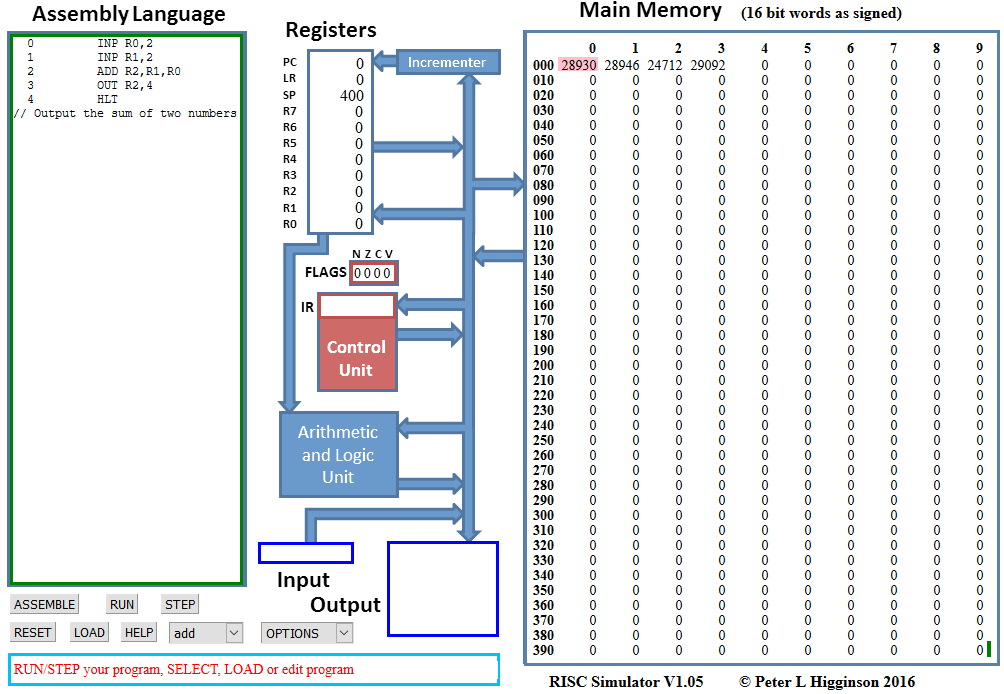
\includegraphics[scale=0.5]{images/RISC.png}
\end{center}

Trois registres ont des fonctions précises.

\begin{itemize}
	\item Le registre PC : Compteur Programme (adresse de la prochaine instruction).
	\item Le registre LR : Adresse de retour (Link Register).
	\item Le registre SP : Pointeur de pile (Stack Pointer).
\end{itemize}

Quatre drapeaux sont représentés (N : Négatif, Z : zéro, C : retenue, V : Dépassement).

\begin{multicols}{3}
\centering

Algorithme

Assembleur

Machine
\end{multicols}

\begin{multicols}{3}
\centering

\begin{algorithm}[H]
$R_1\leftarrow10$\;
\Tq {$R_1\neq0$}
  {   $R_1\leftarrow R_1-1$\;
      Affiche $R_1$\;
  }
\end{algorithm}

\begin{minted}{asm}
        MOV R1,#10
debut:  CMP R1,#0
        BEQ fin
        SUB R1,#1
        OUT R1,4
        BRA debut
fin:    HLT
\end{minted}

\begin{minted}{asm}
0010100100001010
0010000100000000
1000001000000110
0001100100000001
0111000110010100
1000000000000001
0000000000000000
\end{minted}
\end{multicols}

Certaines opérations fondamentales sont disponibles dans la plupart des jeux d'instructions.

\begin{itemize}
	\item Pour le traitement des données. (Calculs arithmétiques, logiques et comparaisons.)
	
	\item Pour le transfert des données (des registres depuis ou vers la mémoire).
	
	\item Pour réaliser des << branchements >>. (Saut non incrémentale d'adresses dans le programme.)
\end{itemize}

Exemples disponibles avec le simulateur : 

(liste complète \href{peterhigginson.co.uk/RISC/instruction_set.pdf}{peterhigginson.co.uk/RISC/instruction\_set.pdf})

\begin{itemize}
	\item Traitement des données.
	
	\asminline{ADD R1,#10} ajoute le nombre 10 au registre R1 ($R_1 \leftarrow R_1+10$),
	
	\asminline{ADD R1,R2,R3} ajoute R3 à R2 et place la somme dans R1 ($R_1 \leftarrow R_1+R_2$),
	
	\asminline{MOV R1, R2} place la valeur de R2 dans R1  ($R_1 \leftarrow R_2$),
	
	\asminline{CMP R1, #27} compare la valeur de R1 avec 27 (Résultats dans les drapeaux).
	
	\item Transfert des données.
   	
	\asminline{STR R1,10} enregistre le contenu du registre R1 en mémoire à l'adresse 10.
   	
	\asminline{LDR R1,10} charge dans le registre R1 le contenu de la mémoire à l'adresse 10.
	
	\item Branchements.
	
	\asminline{BRA 7} saute à l'instruction en mémoire à l'adresse mémoire 7.
	
	\asminline{BRA ici} saute à l'instruction en mémoire à l'adresse du label \asminline{ici:}.
	
	À partir de la valeur des drapeaux, saut d'instruction si
	
	\quad \asminline{BEQ ici} il y a égalité ; \asminline{BNE ici} il n'y a pas égalité
	
	\quad \asminline{BGT ici} la valeur est plus grande ; \asminline{BLT ici} la valeur est plus plus petite.
\end{itemize}


\chapter{Réseau}

\section{Introduction}

\Cours{{\bfseries Réseaux}

Un réseau est un ensemble de \emph{matériels}, connectés de manière à pouvoir \emph{échanger} des données numériques et \emph{partager} des ressources.}


\begin{center}
\begin{tikzpicture}[xscale=1.5]
\coordinate(I)at(0,0);
\coordinate(R0)at($(I)+(1.5cm, 0)$);
\coordinate(C0)at($(R0)+(2cm, -1cm)$);
\coordinate(R)at($(C0)+(-0.75cm, 2cm)$);
\coordinate(C)at($(C0)+(1.5cm, -0.75cm)$);
\coordinate(S0)at($(C0)+(1cm, 1.5cm)$);
\coordinate(S)at($(C0)+(2.5cm, 0.75cm)$);
\coordinate(W)at($(C0)+(-1.5cm, -0.75cm)$);
\coordinate(T)at($(W)+(-1cm, -1.5cm)$);
\coordinate(P)at($(C)+(1.5cm, 0)$);
\coordinate(O1)at($(C)+(-2cm, -1.5cm)$);
\coordinate(O2)at($(C)+(0, -1.5cm)$);
\coordinate(O3)at($(C)+(2cm, -1.5cm)$);
%
\draw(I)--(R0)--(C0)--(S0)(C0)--(S)++(-0.25,1.25)node[right]{\bfseries\large\emph{Réseau local (LAN)}}
     (C0)--(R)--++(-1cm,0)node[left]{liaison étendue WAN}(W)--(C0)--(C)--(P)(C)--(O1)(C)--(O2)(C)--(O3);
\node[cloud, cloud puffs = 15, draw, minimum width = 1.5cm, minimum height = 1.25cm, fill = white]at(I){};
\node[]at(I){\footnotesize Internet};
\node[]at(R0){\routeur};\node[right = 0.5cm]at(R0){routeur};
\node[]at(C0){\switch};\node[right = 0.5cm]at(C0){commutateur};
\node[]at(R){\routeur};\node[right = 0.5cm]at(R){routeur};
\node[]at(C){\switch};\node[left = 0.5cm]at(C){commutateur};
\node[]at(S0){\serveur};\node[right = 0.4cm]at(S0){serveur};
\node[]at(S){\serveur};\node[right = 0.4cm]at(S){serveur};
\node[]at(P){\imprimante};\node[right = 0.4cm, text width=2.5cm]at(P){imprimante\\réseau};
\node[]at(O1){\ordinateur};\node[below = 0.4cm]at(O1){ordinateur};
\node[]at(O2){\ordinateur};\node[below = 0.4cm]at(O2){ordinateur};
\node[]at(O3){\ordinateur};\node[below = 0.4cm]at(O3){ordinateur};
\node[yshift=0.5cm]at(W){\accesWiFi};\node[left = 0.5cm,yshift=0.1cm]at(W){concentrateur WiFi};
\node[]at(T){\telephone};\node[below = 0.4cm]at(T){téléphone};
\draw[](T)++(0.1,0.25)++(20:0.25) arc (20:80:0.25);
\draw[](T)++(0.1,0.25)++(20:0.5) arc (20:80:0.5);
\draw[](T)++(0.1,0.25)++(20:0.75) arc (20:80:0.75);
\end{tikzpicture}
\end{center}

On distingue différents types de réseaux selon leurs tailles (nombre de matériels connectés), leurs structures (façon de les connecter), leurs étendues géographiques (LAN < WAN )...

\noindent\date{1969} Transmission du premier message << login >> sur ARPANET.

(ARPANET - Advanced Research Projects Agency Network - est le premier réseau, développé aux États-Unis, entre des universités.)

\begin{itemize}
	\item en 1981 : 213 machines connectés sur Internet.
	\item en 1989: \np{100000} machines connectés - $1^{\text{er}}$ navigateur web graphique (par le CERN).

(CERN : Conseil européen pour la recherche nucléaire.)
	\item De nos jours, il y en a des dizaines de milliards.
\end{itemize}

\section{Réseaux locaux}

\subsection{Définition}

\Cours{{\bfseries Réseau local (RL) - Local Area Network (LAN)}

C'est un réseau de taille réduite couvrant un domaine privé (entreprises, administrations, universités,...)}

\noindent\date{02/1980} Constitution du comité IEEE  802, pour standardiser les transmissions d'informations.

(IEEE : Institute of Electrical and Electronics Engineers)

En particulier, pour les réseaux locaux :
\begin{multicols}{2}
\begin{itemize}
	\item Ethernet - filaire (IEEE 802.3) ;
	\item 1996 Fast Ethernet (IEEE 802.14) ;
	\item WLAN - réseau sans fil (IEEE 802.11) ;
	\item 2002 Bluetooth (802.15) ; ...
\end{itemize}
\end{multicols}

\subsection{Matériel}

Les réseaux Ethernet sont constitués d'ordinateurs et autres machines possédant une carte réseau, reliés, par des câbles Ethernet, à un ou plusieurs commutateurs (switchs), eux-mêmes reliés entre eux.

\begin{center}\begin{tabular}{ccc}
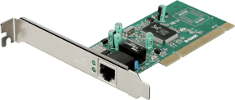
\includegraphics[height=2cm]{images/carteEths.jpg} & 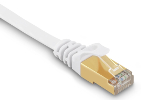
\includegraphics[height=2cm]{images/rj45s.jpg} & 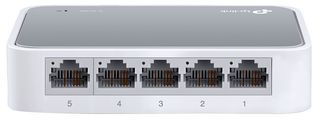
\includegraphics[height=2cm]{images/switch.jpg} \\
carte réseau & câble Ethernet & commutateur (switch) \\
\end{tabular}\end{center}

{\bfseries Pour aller plus loin : } 

Pour relier de tels réseaux entre eux, on utilise des routeurs, possédant, eux, plusieurs cartes réseaux. D'autres supports existent alors, comme la fibre optique.

\begin{center}\begin{tabular}{ccc}
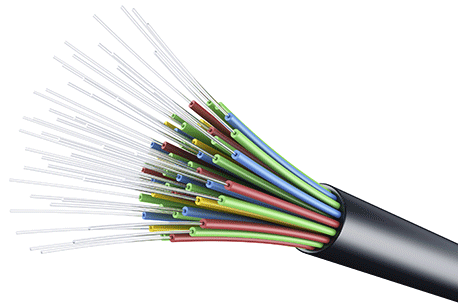
\includegraphics[height=2cm]{images/fibre.png} & 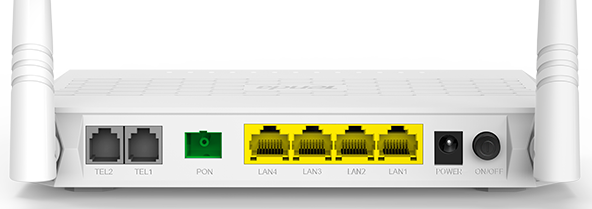
\includegraphics[height=2cm]{images/routeur.png} & 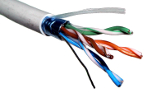
\includegraphics[height=2cm]{images/torsades.jpg}\\
fibre optique & routeur & câble Ethernet \\
\end{tabular}\end{center}

\subsection{Adressage physique (couche Réseau)}

\Cours{{\bfseries Adresse physique (MAC)} (MAC : Media Access Control) 

C'est un identifiant, unique dans le monde, pour chaque carte réseau.}

Elle se présente sous la forme de 6 octets (48 bits), en notation hexadécimale, séparés par un double point ou un tiret. Exemple : \texttt{88-AD-43-F7-26-F8}.

\medskip

Les adresses physiques désignent, dans une \emph{trame}, les protagonistes directs d'un transport de datagramme sur le réseau.

Trame : \fbox{$\cdots$ @MAC-source ; @MAC-destination $\cdots$ \fbox{datagramme} $\cdots$}

C'est chaque bit de cette trame qui est transmis physiquement sur le réseau.

Un \emph{commutateur} (switch) \raisebox{-1ex}{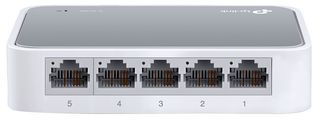
\includegraphics[height=1.5em]{images/switch.jpg}} \raisebox{-1.5ex}{\tikz\node[scale=0.9]{\switch};} est capable de décoder cette trame.
\begin{itemize}
    \item Il met à jour sa liste, appelée \emph{table SAT}, des machines qui lui sont connectées.
    \item Il ne transmet la trame qu'au destinataire.
\end{itemize}


\subsection{Adressage réseaux (couche Internet)}

\Cours{{\bfseries Adresse IP} (IP : Internet Protocol)

 C'est un identifiant (l'adresse), unique dans un réseau (le réseau public : internet, ou un réseau privé), pour chaque carte réseau.}
 
Elle se présente (en version 4) sous la forme de 4 octets (32 bits), en notation décimale, séparés par un  point. Exemple : \texttt{192.168.1.67}

\medskip

On peut demander ses propres identifiants en ligne de commande :

\smallskip

\cmd{ipconfig} (Windows)

\begin{shell}
C:\>ipconfig /all

Carte Ethernet Ethernet:

   Adresse physique . . . . . . . . . . . : 88-AD-43-F7-26-F8
   Adresse IPv4. . . . . . . . . . . . . .: 192.168.1.67
\end{shell}

\smallskip

\cmd{ip} (Unix)

\begin{shell}
moi@ici:~$ ip addr show

2: enp0s3:
    link/ether 88:AD:43:F7:26:F8 brd ff:ff:ff:ff:ff:ff
    inet 192.168.1.67/24 brd 192.168.1.255 scope global dynamic enp0s3
\end{shell}
%$

\medskip

Pour tester si un équipement est joignable sur un réseau IP, on peut utiliser :

\smallskip

\cmd{ping} (Windows / Unix)

\begin{shell}
C:\>ping 192.168.1.1

Envoi d’une requête 'Ping'  192.168.1.1 avec 32 octets de données :
Réponse de 192.168.1.1 : octets=32 temps<1ms TTL=64
...

C:\>ping 192.168.1.7

Envoi d’une requête 'Ping'  192.168.1.7 avec 32 octets de données :
Réponse de 192.168.1.67 : Impossible de joindre l’hôte de destination.
\end{shell}


\medskip

Elle désigne, dans un \emph{datagramme}, les protagonistes initiateur et final et permettent l'acheminement (le routage) de paquets de données. 

Datagramme : \fbox{$\cdots$ @IP-initiale ; @IP-finale $\cdots$ \fbox{paquet}}

C'est l'assemblage de plusieurs paquets qui forme le message envoyé et reçu par les applications.
\subsection{Communication entre applications}


Le but de tout réseau est de pouvoir faire communiquer des logiciels sur des ordinateurs distants. Pour transporter ses données :

\begin{itemize}
	\item l'application fait appel à un protocole de transport : TCP (Transmission Control Protocol) qui va faire des paquets de données (numérotés) à envoyer.
	\item Chaque paquet reçoit l'adresse IP source et l'adresse IP destination,  pour former un datagramme, routable sur internet.
	\item Chaque échange sur les réseaux se fait par trames de données, en identifiant les voisins, de proche en proche, par leur adresse MAC.
\end{itemize}  

\begin{center}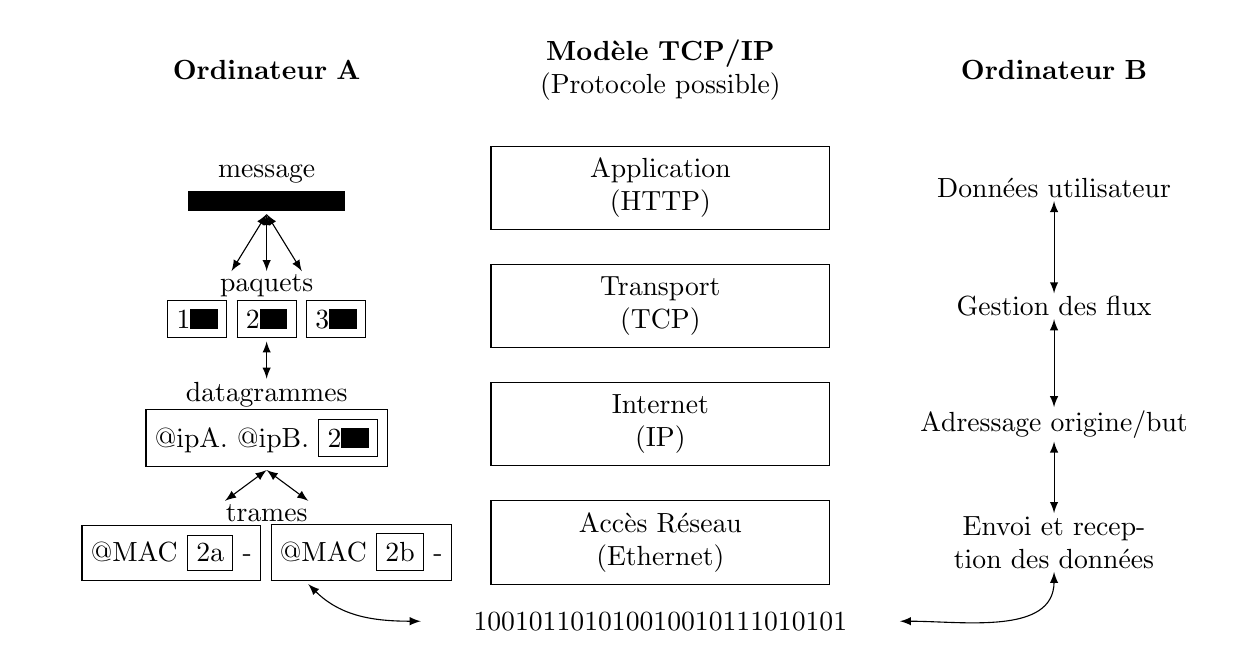
\begin{tikzpicture}[align=center, inner sep=1pt]
\node[text width = 3.5cm, inner sep=1ex](T2){{\bfseries Modèle TCP/IP} \\ (Protocole possible)};
\node[text width = 3.5cm, xshift = -5cm](T1){\bfseries Ordinateur A};
\node[text width = 3.5cm, xshift = 5cm](T3){\bfseries Ordinateur B};
%
\node[text width = 5cm, yshift = -1.5cm](A1)at(T1){message \\ \rule{2cm}{0.25cm}};
\node[text width = 4cm, yshift = -1.5cm, draw, inner sep=1ex](A2)at(T2){Application \\ (HTTP)};
\node[text width = 4cm, yshift = -1.5cm](A3)at(T3){Données utilisateur};
%
\node[text width = 5cm, yshift = -1.5cm](P1)at(A1){paquets \\ \fbox{1\rule{0.35cm}{0.25cm}} \fbox{2\rule{0.35cm}{0.25cm}} \fbox{3\rule{0.35cm}{0.25cm}}};
\node[text width = 4cm, yshift = -1.5cm, draw, inner sep=1ex](P2)at(A2){Transport \\ (TCP)};
\node[text width = 4cm, yshift = -1.5cm](P3)at(A3){Gestion des flux};
%
\node[text width = 5cm, yshift = -1.5cm](I1)at(P1){datagrammes \\ \fbox{@ipA. @ipB. \fbox{2\rule{0.35cm}{0.25cm}}}};
\node[text width = 4cm, yshift = -1.5cm, draw, inner sep=1ex](I2)at(P2){Internet \\ (IP)};
\node[text width = 4cm, yshift = -1.5cm](I3)at(P3){Adressage origine/but};
%
\node[text width = 6cm, yshift = -1.5cm](R1)at(I1){trames \\ \fbox{@MAC \fbox{2a} -} \fbox{@MAC \fbox{2b} -}};
\node[text width = 6cm, yshift = -2.5cm](B)at(I2){$100101101010010010111010101$};
\node[text width = 4cm, yshift = -1.5cm, draw, fill = white, inner sep=1ex](R2)at(I2){Accès Réseau \\ (Ethernet)};
\node[text width = 4cm, yshift = -1.5cm](R3)at(I3){Envoi et reception des données};
%
\draw[latex-latex] (A1.south) -- (P1);
\draw[latex-latex] (A1.south) -- (P1.45);
\draw[latex-latex] (A1.south) -- (P1.135);
\draw[latex-latex] (P1) -- (I1);
\draw[latex-latex] (I1.south) -- (R1.45); 
\draw[latex-latex] (I1.south) -- (R1.135); 
\draw[latex-latex] (R1) to[out=-45,in=180] (B); 
\draw[latex-latex] (A3) -- (P3);
\draw[latex-latex] (P3) -- (I3);
\draw[latex-latex] (I3) -- (R3); 
\draw[latex-latex] (R3) to[out=-90,in=0] (B); 
\end{tikzpicture}\end{center}

{\bfseries Pour aller plus loin : } 

\Cours{{\bfseries Numéro de port} 

 C'est l'identifiant d'une application. Associé à l'adresse IP de l'ordinateur, ils définissent un \emph{socket} qui permet une connexion TCP (Transmission Control Protocol).}
 
 Exemples de ports pré-définis :
 
 \begin{itemize}
 	\item 25 : SMTP (Simple Mail Transfert Protocol)
 	\item 80 : HTTP (HyperText Transfer Protocol)
 	\item 110 : POP3 (Post Office Protocol, version 3) 
 \end{itemize}
 
\subsection{Masque de réseau}

Une adresse IP contient toujours au moins deux informations distinctes : 
\begin{itemize}
	\item l'identifiant du réseau sur lequel est la machine,
	\item et l'identifiant de la machine elle-même sur ce réseau.
\end{itemize}
 
\begin{center}\begin{tikzpicture}
\node[inner sep = 0](IP){\Large\texttt{192.168.1.67}};
\draw[decorate,decoration={brace,raise=0.1cm}](IP.north west) 
     -- ($0.25*(IP.north west)+0.75*(IP.north east)$) node[above=0.2cm,pos=0.2] {Réseau \texttt{192.168.1.0}};
\draw[decorate,decoration={brace,raise=0.1cm}]($0.2*(IP.north west)+0.8*(IP.north east)$)
    node[above right,yshift=0.2cm] {machine  \texttt{67}} -- (IP.north east)  ;
\end{tikzpicture}\end{center}

Plus précisément :

\begin{center}\begin{tikzpicture}
\node[inner sep = 0](IP){\Large\texttt{1100 0000 . 1010 1000 . 0000 0001 . 0100 0011}};
\draw[decorate,decoration={brace,raise=0.1cm}](IP.north west) 
     -- ($0.26*(IP.north west)+0.74*(IP.north east)$) node[above=0.2cm,pos=0.5] {Réseau \texttt{192.168.1.0}};
\draw[decorate,decoration={brace,raise=0.1cm}]($0.205*(IP.north west)+0.795*(IP.north east)$)
     -- (IP.north east)node[above=0.2cm,pos=0.5] {machine  \texttt{67}}  ;
\end{tikzpicture}\end{center}

Mais le nombre de bits attribués au réseau peut être différent, par exemple :

\begin{center}\begin{tikzpicture}
\node[inner sep = 0](IP){\Large\texttt{1100 0000 . 1010 1000 . 0000 0001 . 0100 0011}};
\draw[decorate,decoration={brace,raise=0.1cm}](IP.north west) 
     -- ($0.105*(IP.north west)+0.895*(IP.north east)$) node[above=0.2cm,pos=0.5] {Réseau \texttt{192.168.1.64}};
\draw[decorate,decoration={brace,raise=0.1cm}]($0.095*(IP.north west)+0.905*(IP.north east)$)
     -- (IP.north east)node[above=0.2cm,pos=0.5] {machine  \texttt{3}}  ;
\end{tikzpicture}\end{center}

\Cours{{\bfseries Masque de réseau} 

Le masque d'un réseau se présente sous la forme d'une adresse IP pour laquelle tous les bits composant le réseau sont égaux à 1 et tous les autres égaux à 0.

Elle permet, avec l'opération binaire \pythoninline{&} de déterminer le réseau correspondant à l'adresse IP d'une machine.}

\begin{center}\begin{tikzpicture}
\node[inner sep = 0](IP){\large\texttt{1100 0000 . 1010 1000 . 0000 0001 . 0100 0011}};
\node[inner sep = 0,below=1ex](M)at(IP.south){\large\texttt{1111 1111 . 1111 1111 . 1111 1111 . 1111 0000}};
\node[left=1em]at(M.west){\large\texttt{\&}};
\node[inner sep = 0,below=2ex](R)at(M.south){\large\texttt{1100 0000 . 1010 1000 . 0000 0001 . 0100 0000}};
\draw($(M.south west)+(-2em,-1ex)$)--($(M.south east)+(1em,-1ex)$);
\end{tikzpicture}\end{center}

Sur l'exemple ci-dessus, le masque est \texttt{255.255.255.240}.

Pour simplifier, on peut juste donner le nombre de bits à 1 pour le masque. Par rapport à l'exemple précédent, on peut distinguer \texttt{192.168.1.67/24} et \texttt{192.168.1.67/28} qui ne sont pas sur le même réseau.

Cette distinction est importante car seules les machines partageant le même réseau peuvent communiquer directement ou à travers un commutateur.

\section{Contrôle de flux}

Les messages qui transitent sur les réseaux sont découpés en morceaux (dès la prise en charge par le protocole TCP, qui en fait des paquets). Il peut donc s'avérer important que la source s'assure de la bonne réception de chaque morceau dans le bon ordre pour valider l'envoi (et sinon renvoyer l'information).

On représente la situation par deux axes verticaux représentant l'écoulement du temps au niveau de la source et du destinataire des messages, séparé par un espace représentant le réseau de communication. On symbolise le routage des données par des flèches allant d'une verticale à l'autre. Idéalement :

\begin{center}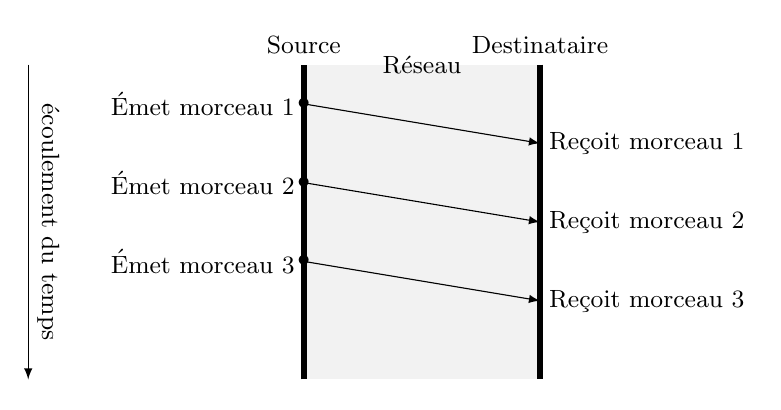
\begin{tikzpicture}\small
\fill[black!5](-1.5cm,-4cm)rectangle(1.5cm,0);
\node{Réseau};
\draw[line width = 2pt](-1.5cm,-4cm)--(-1.5cm,0)node[above]{Source};
\draw[line width = 2pt](1.5cm,0)node[above]{Destinataire}--(1.5cm,-4cm);
\draw[-latex](-1.5cm,-0.5cm)node{$\bullet$}node[left]{Émet morceau 1}--(1.5cm,-1cm)node[right]{Reçoit morceau 1};
\draw[-latex](-1.5cm,-1.5cm)node{$\bullet$}node[left]{Émet morceau 2}--(1.5cm,-2cm)node[right]{Reçoit morceau 2};
\draw[-latex](-1.5cm,-2.5cm)node{$\bullet$}node[left]{Émet morceau 3}--(1.5cm,-3cm)node[right]{Reçoit morceau 3};
\draw[-latex](-5,0)--(-5,-4)node[midway,above,sloped]{écoulement du temps};
\node[]at(0,-3.75){\checkmark};
\end{tikzpicture}\end{center}

On souhaite éviter la perte d'un morceau ou l'arrivée des morceaux dans le désordre :

\begin{center}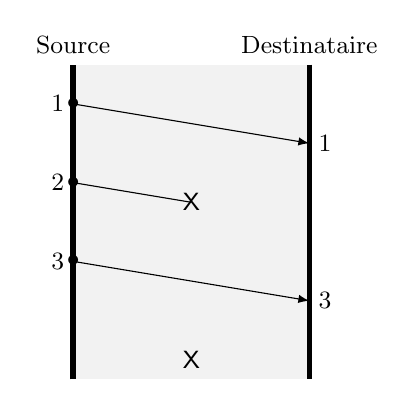
\begin{tikzpicture}\small
\fill[black!5](-1.5cm,-4cm)rectangle(1.5cm,0);
\draw[line width = 2pt](-1.5cm,-4cm)--(-1.5cm,0)node[above]{Source};
\draw[line width = 2pt](1.5cm,0)node[above]{Destinataire}--(1.5cm,-4cm);
\draw[-latex](-1.5cm,-0.5cm)node{$\bullet$}node[left]{1}--(1.5cm,-1cm)node[right]{1};
\draw[-](-1.5cm,-1.5cm)node{$\bullet$}node[left]{2}--(0cm,-1.75cm)node{\textsf{X}};
\draw[-latex](-1.5cm,-2.5cm)node{$\bullet$}node[left]{3}--(1.5cm,-3cm)node[right]{3};
\node[]at(0,-3.75){\textsf{X}};
\end{tikzpicture} \qquad 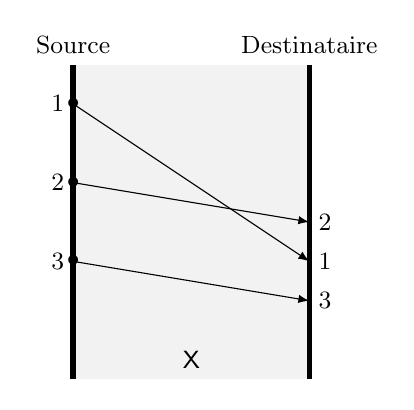
\begin{tikzpicture}\small
\fill[black!5](-1.5cm,-4cm)rectangle(1.5cm,0);
\draw[line width = 2pt](-1.5cm,-4cm)--(-1.5cm,0)node[above]{Source};
\draw[line width = 2pt](1.5cm,0)node[above]{Destinataire}--(1.5cm,-4cm);
\draw[-latex](-1.5cm,-0.5cm)node{$\bullet$}node[left]{1}--(1.5cm,-2.5cm)node[right]{1};
\draw[-latex](-1.5cm,-1.5cm)node{$\bullet$}node[left]{2}--(1.5cm,-2cm)node[right]{2};
\draw[-latex](-1.5cm,-2.5cm)node{$\bullet$}node[left]{3}--(1.5cm,-3cm)node[right]{3};
\node[]at(0,-3.75){\textsf{X}};
\end{tikzpicture}\end{center}

\subsection{Envoyer et attendre (Send and Wait)}

Le principe est le suivant.

\begin{itemize}
	\item La source n'envoie qu'un morceau à la fois et attend un \emph{aquittement} (ACK) du destinataire.
	\item Le destinataire n'envoie un ACK que s'il reçoit un morceau en bon état.
	\item Après un délai pré-établi (timeout) sans ACK, la source renvoie le même morceau.
	\item Après réception d'un ACK, la source envoie le morceau suivant.
\end{itemize}
\begin{center}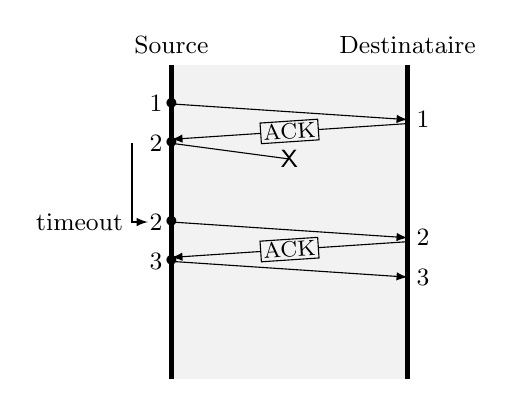
\begin{tikzpicture}\small
\fill[black!5](-1.5cm,-4cm)rectangle(1.5cm,0);
\draw[line width = 2pt](-1.5cm,-4cm)--(-1.5cm,0)node[above]{Source};
\draw[line width = 2pt](1.5cm,0)node[above]{Destinataire}--(1.5cm,-4cm);
\draw[-latex](-1.5cm,-0.5cm)node{$\bullet$}node[left]{1}--(1.5cm,-0.7cm)node[right]{1};
\draw[-latex](1.5cm,-0.75cm)--(-1.5cm,-0.95cm)node[midway,sloped,inner sep=1pt,fill=black!5,draw]{\footnotesize ACK};
\draw[-](-1.5cm,-1cm)node{$\bullet$}node[left]{2}--(0cm,-1.2cm)node{\textsf{X}};
\draw[-latex](-2,-1)--(-2,-2)node[left]{timeout}--(-1.8,-2);
\draw[-latex](-1.5cm,-2cm)node{$\bullet$}node[left]{2}--(1.5cm,-2.2cm)node[right]{2};
\draw[-latex](1.5cm,-2.25cm)--(-1.5cm,-2.45cm)node[midway,sloped,inner sep=1pt,fill=black!5,draw]{\footnotesize ACK};
\draw[-latex](-1.5cm,-2.5cm)node{$\bullet$}node[left]{3}--(1.5cm,-2.7cm)node[right]{3};
\node[]at(0,-3.75){\checkmark};
\end{tikzpicture} \qquad 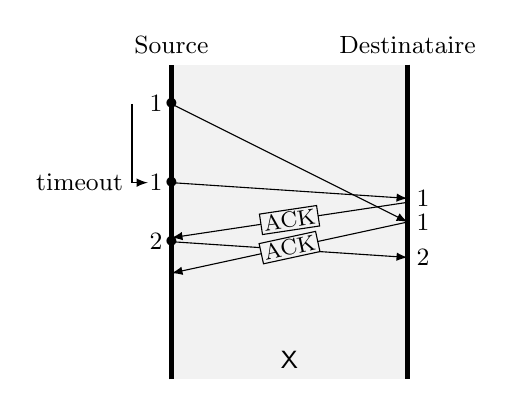
\begin{tikzpicture}\small
\fill[black!5](-1.5cm,-4cm)rectangle(1.5cm,0);
\draw[line width = 2pt](-1.5cm,-4cm)--(-1.5cm,0)node[above]{Source};
\draw[line width = 2pt](1.5cm,0)node[above]{Destinataire}--(1.5cm,-4cm);
\draw[-latex](-1.5cm,-0.5cm)node{$\bullet$}node[left]{1}--(1.5cm,-2cm)node[right]{1};
\draw[-latex](-2,-0.5)--(-2,-1.5)node[left]{timeout}--(-1.8,-1.5);
\draw[-latex](-1.5cm,-1.5cm)node{$\bullet$}node[left]{1}--(1.5cm,-1.7cm)node[right]{1};
\draw[-latex](1.5cm,-1.75cm)--(-1.5cm,-2.2cm)node[midway,sloped,inner sep=1pt,fill=black!5,draw]{\footnotesize ACK};
\draw[-latex](-1.5cm,-2.25cm)node{$\bullet$}node[left]{2}--(1.5cm,-2.45cm)node[right]{2};
\draw[-latex](1.5cm,-2cm)--(-1.5cm,-2.65cm)node[midway,sloped,inner sep=1pt,fill=black!5,draw]{\footnotesize ACK};
\node[]at(0,-3.75){\textsf{X}};
\end{tikzpicture}\end{center}

Ça ne solutionne qu'une partie du problème.

\subsection{Le bit alterné}

Pour mettre de l'ordre dans les morceaux reçus, on ne peut pas vraiment se passer de les numéroter. L'idée du bit alterné, est de ne les numéroter que sur un bit (par économie) que l'on fait alterner entre 0 et 1, en envoi et dans les acquittements.

Notons \texttt{T0} (ou \texttt{T1}) une trame envoyée avec le bit à 0 (ou 1).

L'acquittement demandera la trame suivante en renvoyant le bit opposé: \texttt{A1} (ou \texttt{A0}) l'acquittement correspondant : 

\begin{multicols}{2}
\begin{center}
On résout le problème précédent :

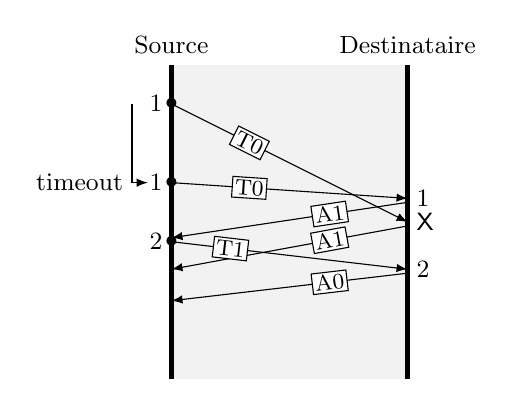
\begin{tikzpicture}\small
% Mise en place
\fill[black!5](-1.5cm,-4cm)rectangle(1.5cm,0);
\draw[line width = 2pt](-1.5cm,-4cm)--(-1.5cm,0)node[above]{Source};
\draw[line width = 2pt](1.5cm,0)node[above]{Destinataire}--(1.5cm,-4cm);
% Première trame
\draw[-latex](-1.5cm,-0.5cm)node{$\bullet$}node[left]{1}--(1.5cm,-2cm)node[pos=0.33,sloped,inner sep=1pt,fill=white,draw]{\footnotesize T0}node[right]{\textsf{X}};
\draw[-latex](-2,-0.5)--(-2,-1.5)node[left]{timeout}--(-1.8,-1.5);
% Première trame bis
\draw[-latex](-1.5cm,-1.5cm)node{$\bullet$}node[left]{1}--(1.5cm,-1.7cm)node[pos=0.33,sloped,inner sep=1pt,fill=white,draw]{\footnotesize T0}node[right]{1};
\draw[-latex](1.5cm,-1.75cm)--(-1.5cm,-2.2cm)node[pos=0.33,sloped,inner sep=1pt,fill=white,draw]{\footnotesize A1};
\draw[-latex](1.5cm,-2.05cm)--(-1.5cm,-2.6cm)node[pos=0.33,sloped,inner sep=1pt,fill=white,draw]{\footnotesize A1};
% Seconde trame
\draw[-latex](-1.5cm,-2.25cm)node{$\bullet$}node[left]{2}--(1.5cm,-2.6cm)node[pos=0.25,sloped,inner sep=1pt,fill=white,draw]{\footnotesize T1}node[right]{2};
\draw[-latex](1.5cm,-2.65cm)--(-1.5cm,-3cm)node[pos=0.33,sloped,inner sep=1pt,fill=white,draw]{\footnotesize A0};
\node[]at(0,-3.75){\checkmark};
\end{tikzpicture}


Mais pas tous les problèmes :

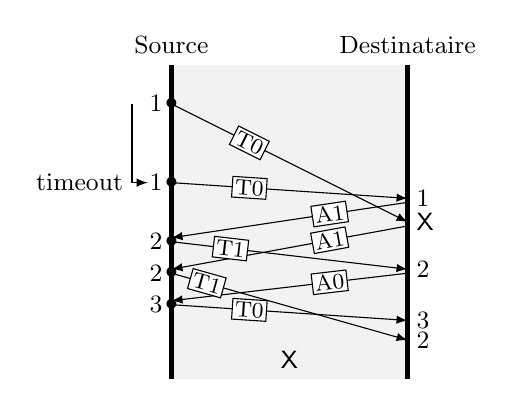
\begin{tikzpicture}\small
% Mise en place
\fill[black!5](-1.5cm,-4cm)rectangle(1.5cm,0);
\draw[line width = 2pt](-1.5cm,-4cm)--(-1.5cm,0)node[above]{Source};
\draw[line width = 2pt](1.5cm,0)node[above]{Destinataire}--(1.5cm,-4cm);
% Première trame
\draw[-latex](-1.5cm,-0.5cm)node{$\bullet$}node[left]{1}--(1.5cm,-2cm)node[pos=0.33,sloped,inner sep=1pt,fill=white,draw]{\footnotesize T0}node[right]{\textsf{X}};
\draw[-latex](-2,-0.5)--(-2,-1.5)node[left]{timeout}--(-1.8,-1.5);
% Première trame bis
\draw[-latex](-1.5cm,-1.5cm)node{$\bullet$}node[left]{1}--(1.5cm,-1.7cm)node[pos=0.33,sloped,inner sep=1pt,fill=white,draw]{\footnotesize T0}node[right]{1};
\draw[-latex](1.5cm,-1.75cm)--(-1.5cm,-2.2cm)node[pos=0.33,sloped,inner sep=1pt,fill=white,draw]{\footnotesize A1};
\draw[-latex](1.5cm,-2.05cm)--(-1.5cm,-2.6cm)node[pos=0.33,sloped,inner sep=1pt,fill=white,draw]{\footnotesize A1};
% Seconde trame
\draw[-latex](-1.5cm,-2.25cm)node{$\bullet$}node[left]{2}--(1.5cm,-2.6cm)node[pos=0.25,sloped,inner sep=1pt,fill=white,draw]{\footnotesize T1}node[right]{2};
\draw[-latex](1.5cm,-2.65cm)--(-1.5cm,-3cm)node[pos=0.33,sloped,inner sep=1pt,fill=white,draw]{\footnotesize A0};
% Seconde trame bis
\draw[-latex](-1.5cm,-2.65cm)node{$\bullet$}node[left]{2}--(1.5cm,-3.5cm)node[pos=0.15,sloped,inner sep=1pt,fill=white,draw]{\footnotesize T1}node[right]{2};
% Troisième trame
\draw[-latex](-1.5cm,-3.05cm)node{$\bullet$}node[left]{3}--(1.5cm,-3.25cm)node[pos=0.33,sloped,inner sep=1pt,fill=white,draw]{\footnotesize T0}node[right]{3};
\node[]at(0,-3.75){\textsf{X}};
\end{tikzpicture}
\end{center}
\end{multicols}

{\bfseries Pour aller plus loin : } Au niveau du protocole TCP, chaque segment porte un numéro de séquence et un numéro d'acquittement, chacun sur 32 bit pour assurer la bonne réception de l'ensemble dans le bon ordre. 

Par comparaison, le protocole UDP (sans connexion) n'en utilise aucun, pour gagner en rapidité. (Dans un flux vidéo par exemple perdre une partie d'une image est moins grave que de faire une pause pour l'attendre.)

\chapter{Système d'exploitation}

\section{Fonctions d'un système d'exploitation}

\begin{multicols}{2}\Cours{{\bfseries Système d'exploitation}


Un système d'exploitation est l'interface logicielle entre les applications et le matériel informatique. }

(Les utilisateurs utilisent les applications, qui demandent des ressources au système d'exploitation, qui pilote le matériel informatique, le partageant entre différentes applications et différents utilisateurs.)



\begin{tikzpicture}\node[scale=0.49]{\begin{tikzpicture}
\draw[fill=black!5, rounded corners = 5pt](-3,-2.25)rectangle(11,1.25);
\node[text width = 3cm, draw, align=center](A){\raisebox{-1ex}{\rule{0pt}{4ex}}Processeur};
\node[text width = 3cm, draw, align=center, xshift=2.5cm](B)at(A.east){\raisebox{-1ex}{\rule{0pt}{4ex}}Mémoire};
\node[text width = 3cm, draw, align=center, xshift=2.5cm](C)at(B.east){\raisebox{-1ex}{\rule{0pt}{4ex}}Entrées/Sorties};
\node[text width = 12cm, draw, align=center, yshift=-1cm, double arrow](D)at(B.south){Bus de communication};
\draw(A.south)--++($(D.north)-(B.south)$);
\draw(B.south)--++($(D.north)-(B.south)$);
\draw(C.south)--++($(D.north)-(B.south)$);
\node[above=0,inner sep = 0]at(B.north){\huge \bfseries Matériel informatique};
\draw[fill=black!5, rounded corners = 5pt](-3,1.75)rectangle(11,3.25);
\draw[fill=white, rounded corners = 5pt](-2.9,1.85)rectangle(10.9,3.15)node[midway]{\huge \bfseries Système d'exploitation};
\draw[fill=black!5, rounded corners = 5pt](-3,3.75)rectangle(11,5.25)node[midway]{{\huge \bfseries Applications} (processus)};
\draw[fill=black!5, rounded corners = 5pt](-3,5.75)rectangle(11,7.25)node[midway]{{\huge \bfseries Utilisateurs}};
\foreach \x in {0,0.5,...,5} \draw[-latex]({-2.25+\x},1.75)--({-2.25+\x},1.25);
\foreach \x in {0,0.5,...,5} \draw[-latex]({5.25+\x},1.25)--({5.25+\x},1.75);
\foreach \x in {0,0.5,...,5} \draw[-latex]({-2.25+\x},3.75)--({-2.25+\x},3.25);
\foreach \x in {0,0.5,...,5} \draw[-latex]({5.25+\x},3.25)--({5.25+\x},3.75);
\foreach \x in {0,0.5,...,5} \draw[-latex]({-2.25+\x},5.75)--({-2.25+\x},5.25);
\foreach \x in {0,0.5,...,5} \draw[-latex]({5.25+\x},5.25)--({5.25+\x},5.75);
\end{tikzpicture}};
\end{tikzpicture}\end{multicols}

Il existe différentes familles de systèmes d'exploitations.

\noindent\date{1970} Naissance d'UNIX, père des systèmes d'exploitation modernes (macOS, iOS
, Android, Linux sont de la famille UNIX). UNIX étant un système propriétaire (les sources appartiennent à une entreprise et ne sont pas publiques), c'est en clonant ce système (sans utiliser ses sources) que Linux a été écrit (1991).

\noindent\date{1985} Naissance de Windows (sur MS-DOS). Mais il en existe bien d'autres...

\medskip

On peut distinguer quatre grands types de fonctions (trois directement liées au matériel).

\begin{itemize}
	\item La gestion des processus.
	\item La gestion de la mémoire.
	\item La gestion des périphériques d'entrée/sortie.
	\item La gestion du système de fichiers.
\end{itemize}

\section{IHM et Ligne de commande}

\Cours{{\bfseries Interface Homme-Machine}

Une Interface Homme-Machine - IHM est un ensemble de mécanismes, à la fois matériels et logiciels, mis à la disposition des utilisateurs pour leur permettre d'interagir avec un système interactif.}

Cette interface est mise en œuvre sur un \emph{terminal}, ensemble de périphériques d'entrée / sortie, à l'extrémité d'un ordinateur ou d'un réseau. Souvent intégré (clavier, écran tactile, \ldots) mais pas toujours (Terminal bancaire), il peut aussi être virtuel (console  d'un système d'exploitation).

\begin{center}


\includegraphics[height=2cm]{images/clavier-cles-ordinateur-portable-93422.jpg}\quad
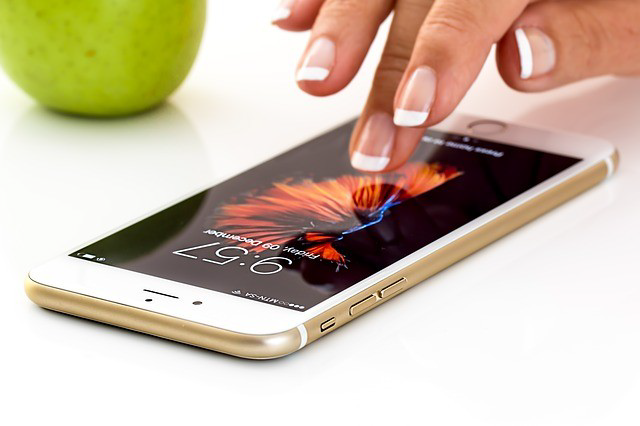
\includegraphics[height=2cm]{images/ecrant.png}\quad
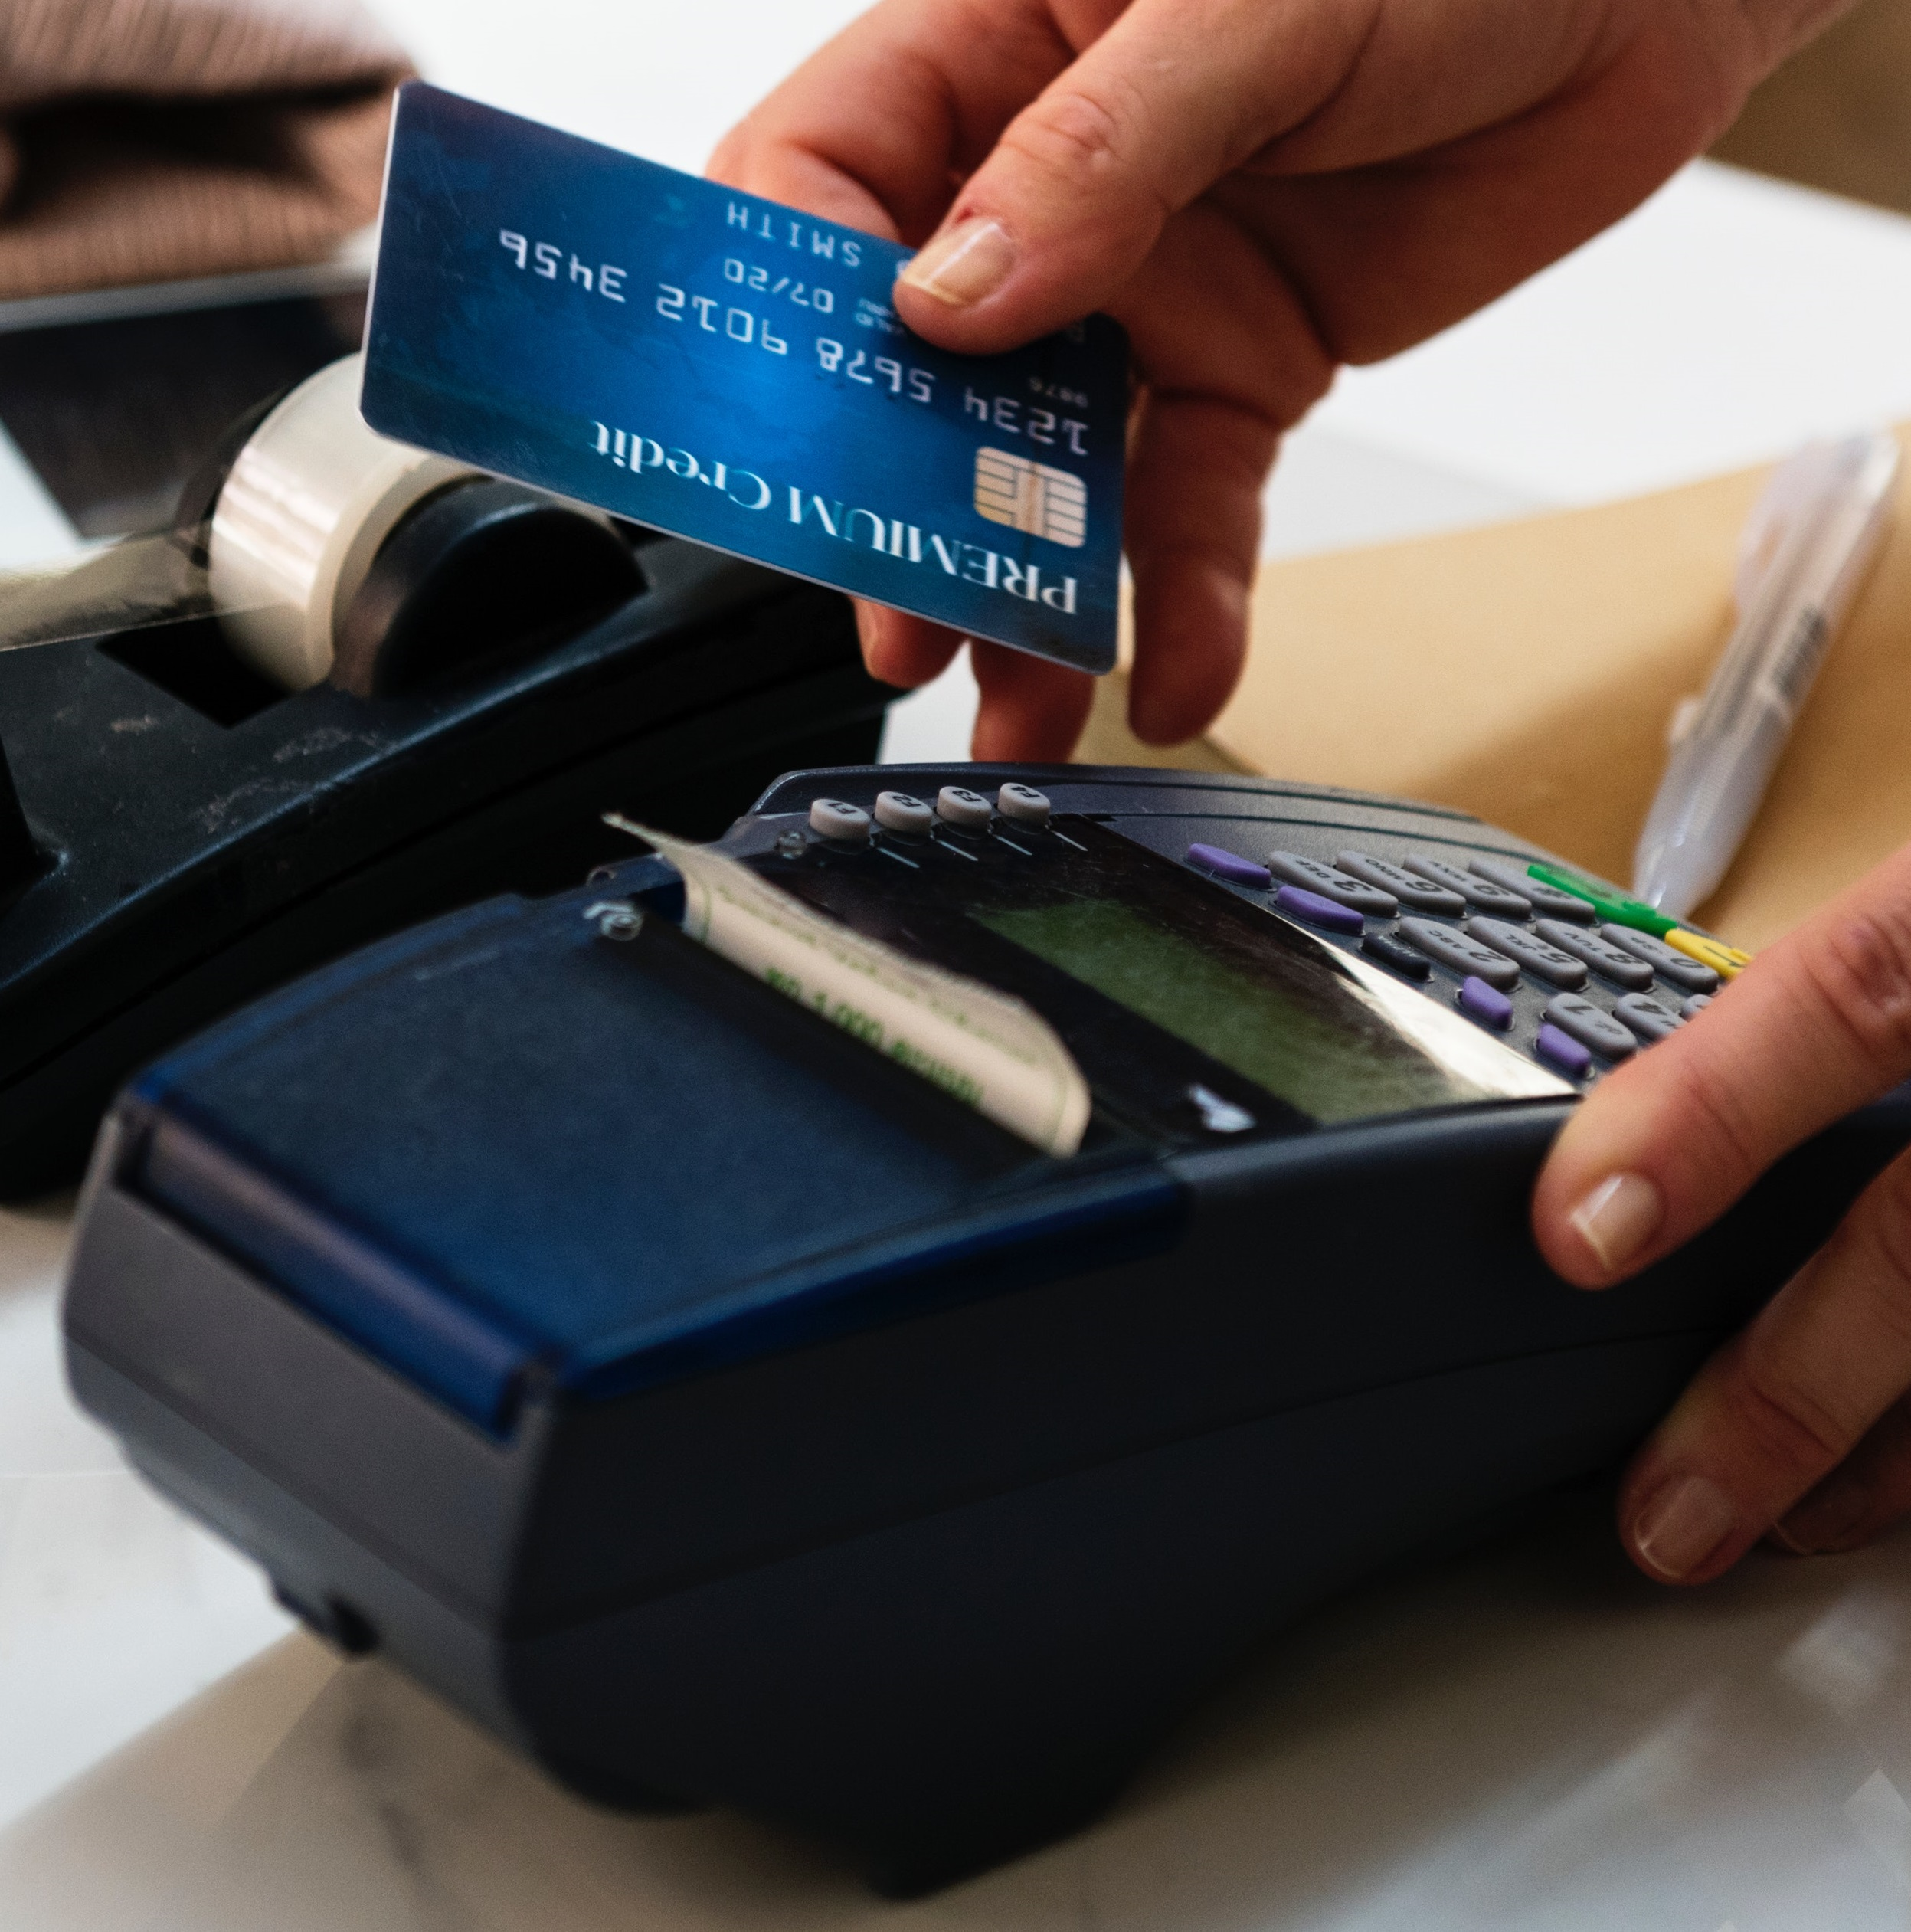
\includegraphics[height=2cm]{images/access-card-cellphone.jpg}\quad
%https://commons.wikimedia.org/wiki/File:Credit_card_terminal_in_Laos.jpg

\includegraphics[height=2cm]{images/bash-148836_960_720}
	
\end{center} 

Sous Ubuntu, c'est l'application  \mintinline{text}{Terminal} ; sous Windows, \mintinline{text}{cmd}.

\begin{multicols}{2}
\noindent\begin{shell}
moi@mongroupe:~$
\end{shell}
%$

L'invite de commande Ubuntu se compose du nom d'utilisateur, de \mintinline{text}{@} et de son groupe, suivi de \mintinline{text}{:} ,
 du répertoire courant (\mintinline{text}{~} pour le répertoire utilisateur) et termine par \mintinline{text}{$}.%$
\columnbreak

\noindent\begin{shell}
C:\Users\moi>
\end{shell}

L'invite de commande << MS-DOS >> de Windows se compose du nom du lecteur, suivi de \mintinline{text}{:}, du répertoire courant et termine par \mintinline{text}{>}.%$
\end{multicols}
%(Exemple motivant : (Win) \texttt{> ren IMG*.jpg ete2019*.jpg})

Une commande est alors composée d'un nom suivi ou non d'options. Les commandes spécifiques au système (que ce soit Ubuntu ou Windows) sont listées par la commande \cmd{help}

Pour effacer la console par exemple : \cmd{clear} (UNIX) ou \cmd{cls} (Windows).

\subsection{Navigation dans l'arborescence des fichiers}

Les données en mémoire sont répertoriées par des fichiers, caractérisés par leur nom, taille, droit d'accès, propriétaire, date de création, de modification, \ldots Ces fichiers sont eux-mêmes répertoriés dans une structure arborescente dont chaque nœud est un dossier. Dans un système UNIX, tout part d'une même racine (root) : \mintinline{text}{/}. Dans un système Windows, il y a une arborescence par disque logique, identifiée par une lettre.

\begin{multicols}{2}
\begin{center}
UNIX

\begin{tikzpicture}
\node(racine)at(0,0){\mintinline{text}{/}};
\node[below left = 1cm, xshift=-0.5cm](bin)at(racine){\mintinline{text}{bin}};
\node[below right = 1cm, xshift=0.5cm](media)at(racine){\mintinline{text}{media}};
\node(home)at($0.5*(bin)+0.5*(media)$){\mintinline{text}{home}};
\node[]at($0.5*(bin)+0.5*(home)$){\ldots};
\node[]at($0.5*(home)+0.5*(media)$){\ldots};
\draw(racine)--(bin);
\draw(racine)--(home);
\draw(racine)--(media);
\draw(bin)++(-0.2cm,-0.75cm)--++(-0.5cm,-0.5cm);
\draw(bin)++(0,-0.75cm)--++(0cm,-0.5cm);
\draw(bin)++(0.2cm,-0.75cm)--++(0.5cm,-0.5cm);
\draw(home)++(-0.2cm,-0.5cm)--++(-0.5cm,-0.75cm);
\draw(home)++(0,-0.5cm)--++(0cm,-0.75cm);
\draw(home)++(0.2cm,-0.5cm)--++(0.5cm,-0.75cm);
\draw(media)++(-0.2cm,-0.75cm)--++(-0.5cm,-0.5cm);
\draw(media)++(0,-0.75cm)--++(0cm,-0.5cm);
\draw(media)++(0.2cm,-0.75cm)--++(0.5cm,-0.5cm);
\node[below=3pt](bin1)at(bin){\scriptsize commandes};\node[below]at(bin1){\scriptsize UNIX};
\node[below=3pt]at(home){\scriptsize utilisateurs};
\node[below=3pt](media1)at(media){\scriptsize supports};\node[below]at(media1){\scriptsize amovibles};
\end{tikzpicture}

Windows

\begin{tikzpicture}
\node(C)at(0,0){\mintinline{text}{C:\}};
\node[below left = 1cm, xshift=0.2cm](W)at(C){\mintinline{text}{Windows}};
\node[below right = 1cm, xshift=-0.2cm](U)at(C){\mintinline{text}{Users}};
\node[]at($0.5*(W)+0.5*(U)$){\ldots};
\draw(C)--(W);
\draw(C)--(U);
\draw(W)++(-0.2cm,-0.5cm)--++(-0.5cm,-0.75cm);
\draw(W)++(0,-0.5cm)--++(0cm,-0.75cm);
\draw(W)++(0.2cm,-0.5cm)--++(0.5cm,-0.75cm);
\draw(U)++(-0.2cm,-0.5cm)--++(-0.5cm,-0.75cm);
\draw(U)++(0,-0.5cm)--++(0cm,-0.75cm);
\draw(U)++(0.2cm,-0.5cm)--++(0.5cm,-0.75cm);
\node[below=3pt]at(W){\scriptsize système};
\node[below=3pt]at(U){\scriptsize utilisateurs};
\node[right=2.5cm](I)at(C){\mintinline{text}{I:\}};
\draw(I)++(-0.2cm,-0.5cm)--++(-0.4cm,-0.5cm);
\draw(I)++(0,-0.5cm)--++(0cm,-0.5cm);
\draw(I)++(0.2cm,-0.5cm)--++(0.4cm,-0.5cm);
\node[below=3pt]at(I){\scriptsize support amovible};
\end{tikzpicture}\end{center}
\end{multicols}

\begin{center}
\begin{tabular}{L{1.5cm}L{3cm}L{7cm}}
UNIX & Windows & Action \\
\hline
\cmd{pwd} & \cmd{cd} & Affiche le répertoire courant \\
\cmd{cd} & \cmd{cd \%HOMEPATH\%} & Positionne au répertoire utilisateur \\
\cmd{cd ..} & \cmd{cd ..} & Positionne au répertoire parent \\
\cmd{cd /} & \cmd{cd \textbackslash } & Positionne à la racine \\
\end{tabular}
\end{center}

De manière générale : \cmd{cd} suivi d'un chemin positionne au bout du chemin.

Le chemin peut être \emph{relatif} (au répertoire courant) ou \emph{absolu} (commençant par \cmd{/} ou \cmd{C:\textbackslash}).

\cmd{..} est le répertoire précédent, \cmd{.} le répertoire courant.

La touche de tabulation permet une complétion automatique des noms de fichiers.

\medskip

\begin{center}
\begin{tabular}{L{1.5cm}L{2.5cm}L{7cm}}
UNIX & Windows & Action \\
\hline
\cmd{ls} & \cmd{dir} & Liste les fichiers du répertoire courant \\
\end{tabular}
\end{center}

En faisant suivre le nom d'une commande par \cmd{-h} ou \cmd{-{}-help} (UNIX) ou \cmd{/?} (Windows), on obtient des détails sur leurs utilisations et options. Par exemple, pour obtenir une liste récursive des fichiers du répertoire courant et de ses sous-répertoires : \cmd{ls -R}  ou \cmd{dir /S}.

\medskip

Autres actions possibles sur les dossiers :

\begin{center}
\begin{tabular}{L{3cm}L{3cm}L{7cm}}
UNIX & Windows & Action \\
\hline
\cmd{mkdir monRep} & \cmd{md monRep} & Crée le répertoire \mintinline{text}{monRep} \\
\cmd{mv monRep rep} & \cmd{ren monRep rep} & Renomme le répertoire \mintinline{text}{monRep} en \mintinline{text}{rep}  \\
\cmd{rmdir monRep} & \cmd{rd monRep} & Supprime le répertoire vide \mintinline{text}{monRep} \\
\end{tabular}
\end{center}

\subsection{Visualisation et manipulation des fichiers}

Quelques actions possibles sur les fichiers :

\begin{center}
\begin{tabular}{L{5cm}L{5cm}L{3cm}}
UNIX & Windows & Action \\
\hline
\cmd{touch fichier.txt} & Pas d'équivalent$^\star$ & Crée\\
\cmd{cat fichier.txt} & \cmd{type fichier.txt} & Affiche le contenu\\
\cmd{mv fichier.txt test.txt} & \cmd{ren fichier.txt test.txt} & Renomme\\
\cmd{mv test.txt monRep} & \cmd{move test.txt monRep} & Déplace\\
\cmd{cp test.txt monRep} & \cmd{copy test.txt monRep} & Copie\\
\cmd{rm test.txt} & \cmd{del test.txt} & Supprime \\
\end{tabular}

($^\star$ {\small Dans le cas où le fichier n'existe pas déjà on peut écrire \cmd{type Nul > fichier.txt}})
\end{center}

\medskip

On peut lancer des applications depuis la ligne de commande. 

Exemples: \cmd{gedit fichier.txt} (UNIX) ou \cmd{notepad fichier.txt} (Window).

\section{Droits et permissions d'accès aux fichiers}

Sous Windows, il n'existe pas vraiment d'équivalent aux lignes de commandes proposées ci-dessous. On ne considère donc ici que les fichiers d'un système de type UNIX. On les distingue par :

\begin{multicols}{3}
\begin{itemize}
	\item 4 types de fichier 
	
		\cmd{-} Ordinaire
		
		\cmd{d} Répertoire (directory) 
		
		\cmd{l} Lien symbolique (link)
		
		\cmd{c} ou \cmd{b} Spécial
	\item 3 catégories 
	
	d'utilisateurs 
	
	\cmd{u} Propriétaire (user)
	
	 \cmd{g} Groupe (group)
	 
	  \cmd{o} Autres (others)
	\item 3 types de droit 
	
	 \cmd{r} Lecture (read)
	 
	  \cmd{w} Écriture (write)
	  
	  \cmd{x} Exécution (execute)
\end{itemize}
\end{multicols}

On peut visualiser ces informations par un listing détaillé : \cmd{ls -l}.

\medskip Les trois types de droit pouvant ou non être accordés indépendamment, ils génèrent $2^3=8$ possibilités, que l'on numérote comme s'ils écrivaient un nombre binaire :

\begin{center}
\begin{tabular}{cccccccc}
\cmd{-{}-{}-} &\cmd{-{}-{}x} &\cmd{-w-} &\cmd{-wx} &\cmd{r-{}-} &\cmd{r-x} &\cmd{rw-} &\cmd{rwx}  \\
\hline 
$0$ & $1$ & $2$ & $3$ & $4$ & $5$ & $6$ & $7$  \\
\end{tabular}
\end{center}

En juxtaposant les droits des 3 catégories d'utilisateurs, on obtient alors un nombre écrit en octal.

Exemple : Un répertoire \cmd{d}, pour lequel le  propriétaire a tous les droits \cmd{rwx}, que le groupe n'a juste pas le droit de modifier \cmd{r-x} et qui ne laisse le droit qu'en lecture aux autres \cmd{r-{}-} est de type \cmd{drwxr-xr-{}-}. Ces droits se lisent en octal : $754$.

\medskip

On peut changer les droits en donnant sa valeur en octal :

\cmd{chmod 777 fichier.txt} donne tous les droits à tout le monde sur le fichier.

\medskip

On peut modifier les droits relativement à certains utilisateurs :

\cmd{chmod o - w fichier.txt} enlève le droit d'écriture aux autres utilisateurs.

(o peut être g ou u, - peut être + et w peut être r ou x)





\chapter{Exemple concret d'un nano-ordinateur}

On prend ici l'exemple du nano-ordinateur micro\string:bit.

\begin{center}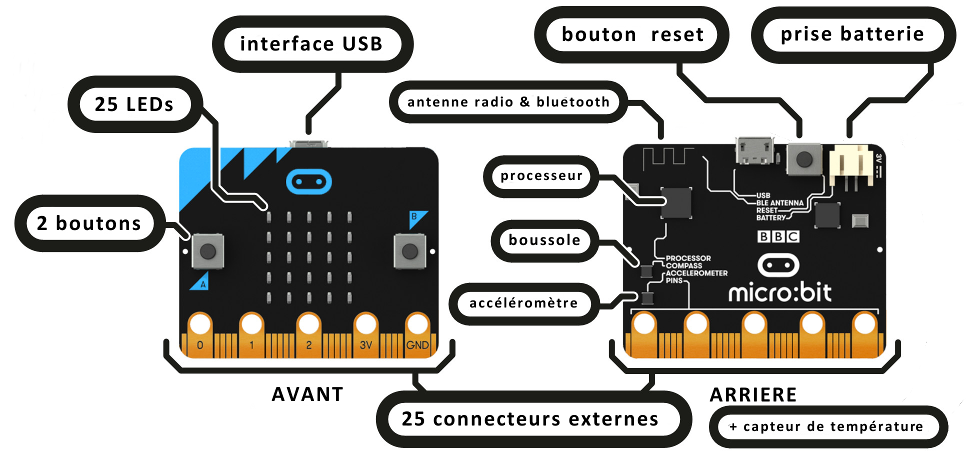
\includegraphics[width=0.95\linewidth]{images/microbit-hardware-access-fr.png}\end{center}

On utilise l'IDE Mu qui permet facilement de flasher la carte, et la bibliothèque dédiée :

\begin{minted}{python3}
from microbit import *
\end{minted}

On pourra trouver une introduction et des précisions sur le langage MicroPython utilisé :

\href{https://microbit-micropython.readthedocs.io/fr/latest/tutorials/introduction.html}{https://microbit-micropython.readthedocs.io/fr/latest/tutorials/introduction.html}

\section{Capteurs et actionneurs}

\Cours{{\bfseries Capteur}

Un capteur est un périphérique d'entrée. Il permet l'acquisition d'une grandeur physique (température, luminosité, présence, distance, \ldots), qu'il transforme en un signal électrique (logique, analogique ou numérique) qui pourra être traité par le reste du système.
}

Par exemple, avec la micro\string:bit :

\begin{itemize}
	\item Deux boutons \pythoninline{button_a} et \pythoninline{button_b} de méthodes :
	
	\begin{tabular}{ll}
	\pythoninline{is_pressed()} & renvoie \pythoninline{True} ou \pythoninline{False} selon si le bouton A est enfoncé,  \\
	\pythoninline{was_pressed()} & renvoie \pythoninline{True} ou \pythoninline{False} selon si le bouton A a été appuyé et relâché, \\
	\pythoninline{get_presses()} & renvoie et remet à zéro le nombre de fois où A a été appuyé. \\
	\end{tabular}
    \item Un accéléromètre \pythoninline{accelerometer} de méthodes :

	\begin{tabular}{ll}
	\pythoninline{get_x()} & renvoie un entier relatif indiquant la direction selon l'axe (Ox),  \\
	\pythoninline{get_y()} & renvoie un entier relatif indiquant la direction selon l'axe (Oy), \\
	\pythoninline{get_z()} & renvoie un entier relatif indiquant la direction selon l'axe (Oz), \\
	\pythoninline{get_values()} & renvoie un triplet d'entiers relatifs indiquant la direction (x,y,z),  \\
	\pythoninline{current_gesture()} & renvoie le nom du geste en cours.  \\
	\end{tabular}
	
	MicroPython comprend les gestes :  \pythoninline{"up"}, \pythoninline{"down"}, \pythoninline{"left"}, \pythoninline{"right"}, 
	
	\pythoninline{"face up"}, \pythoninline{"face down"}, \pythoninline{"freefall"}, \pythoninline{"3g"}, \pythoninline{"6g"}, \pythoninline{"8g"}, \pythoninline{"shake"}.
	
	
    \item Une boussole \pythoninline{compass} de méthodes :
    \pythoninline{calibrate()} (indispensable en début d'utilisation), \pythoninline{is_calibrated()} et \pythoninline{clear_calibration()}.
    
    \pythoninline{get_x()}, \pythoninline{get_y()}, \pythoninline{get_z()} comme pour l'accéléromètre.
    
    \pythoninline{heading()} qui renvoie un angle entier positif en degrés (0 pour le nord à 360).
    
    \pythoninline{get_field_strength()} qui renvoie un entier représentant l'intensité magnétique.
    \item Un capteur de température, donnée par \pythoninline{temperature()}.
\end{itemize}

\Cours{{\bfseries Actionneur}

Un actionneur est un périphérique de sortie. Il permet la conversion de l'énergie (électrique) en une action physique (mécanique, lumineuse, \ldots).
}

La micro\string:bit seule ne possède qu'un actionneur : une grille de LED 5$\times$5 : \pythoninline{display}.

Ses méthodes principales :

\begin{itemize}
	\item \pythoninline{get_pixel(x, y)} renvoie un entier entre 0 et 9 d'intensité lumineuse,
	\item \pythoninline{set_pixel(x, y, valeur)} règle l'intensité lumineuse par une valeur entre 0 et 9,
	\item \pythoninline{clear()} règle toutes les intensités lumineuses à 0,
	\item \pythoninline{show(value, delay=400, wait=True, loop=False, clear=False)} :
	 
	\pythoninline{value} peut être un nombre, une chaine  de caractères, une image ou une liste d'images.
	
	Une image pouvant être l'une des images prédéfinies, \pythoninline{Image.HEART}, \pythoninline{Image.HEART_SMALL}, \pythoninline{Image.HAPPY}, \pythoninline{Image.SMILE}, \pythoninline{Image.SAD} \ldots ou créée en indiquant l'intensité lumineuse de chaque LED (de gauche à droite et de haut en bas) :
	
    \pythoninline{image = Image("90009:09090:00900:09090:90009")}.
	
	\pythoninline{delay} est le temps en microsecondes entre deux images d'une liste.
	
	\pythoninline{wait} bloque l'exécution si \pythoninline{True}, affiche en tache de fond si \pythoninline{False}.
	
	\pythoninline{loop} détermine s'il y a répétition ou non.
	
	\pythoninline{clear} détermine si l'affichage est effacé après l'exécution. 
	\item \pythoninline{scroll(value, delay=150, wait=True, loop=False, monospace=False)}.
	
\end{itemize}

\section{Réalisation d'une Interface Homme Machine}

Si l'on veut faire se déplacer un point lumineux selon l'inclinaison de la carte et terminer en fixant sa position, on a besoin de :

\begin{itemize}
	\item initialiser la position. Par exemple au centre : \pythoninline{x = 3} et \pythoninline{y = 3}.
	\item utiliser une boucle qui ne s'arrête que si l'utilisateur le demande par une action,
	      
	       Par exemple : \pythoninline{while not button_a.is_pressed() :}
	\item lire les données du bon capteur.
	
	Ici : \pythoninline{accelerometer.get_x()} et \pythoninline{accelerometer.get_y()}.
	
	\item utiliser ces données pour mettre à jour les variables du programme.
	
	\item agir sur le bon actionneur en fonction de cette mise à jour.
	
	Ici : \pythoninline{display.set_pixel(int(x),int(y),9)} 
	
\end{itemize}

Ce qui donne finalement :

\begin{minted}{python}
from microbit import *

x = 3
y = 3
while not button_a.is_pressed() :
    x = x + accelerometer.get_x() / 1000
    y = y + accelerometer.get_y() / 1000
    if(x>4): x = 4
    if(x<0): x = 0
    if(y>4): y = 4
    if(y<0): y = 0
    sleep(100)
    display.clear()
    display.set_pixel(int(x),int(y),9)
\end{minted}













%(robot : Micro\string:Maqueen ? )